\documentclass[11pt,aspectratio=169,
xcolor={table},
hyperref={
hidelinks,
pdfauthor={Peter Schulz},
pdftitle={Infromatik am Abgrund - Klettern in Virtueller Realität},
pdfsubject={Master Thesis},
pdfkeywords={Sport Climbing;Virtual Reality;Mixed Reality;Passive Haptics;Presence},
pdfencoding=auto},
url={obeyspaces,spaces,hyphens}]{beamer}

\usepackage{polyglossia,csquotes}
\setdefaultlanguage{german}

\usetheme[numbering=fraction]{metropolis}
\usepackage{appendixnumberbeamer}

\usepackage{booktabs}
\usepackage[scale=2]{ccicons}

\usepackage{caption,subcaption}
\usepackage[percent]{overpic}

\usepackage{fontawesome}
\usepackage{cancel}

\usepackage{graphicx,graphbox}
\usepackage[percent]{overpic}

\usepackage[absolute,overlay]{textpos}
\setlength{\TPHorizModule}{1mm}
\setlength{\TPVertModule}{1mm}

\usepackage{luatex85,fontspec,xspace}

\usepackage{multimedia}

\usepackage[onlymath]{MinionPro}

\usepackage[
natbib,
maxnames=4,
maxcitenames=2,
maxbibnames=4,
maxitems=2,
uniquelist=false,
style=authoryear-comp,
backend=biber,
sorting=anyt,
sortcites=false,
sortlocale=en_US,
hyperref=true,
url=false,
isbn=false,
backref=false,
giveninits=true,
block=none]{biblatex}
\bibliography{../../master-thesis/tex/master-thesis}

\usepackage[xindy,acronym,style=index,nonumberlist,seeautonumberlist,toc]{glossaries}
\makeglossaries

% Define "long-ing" key: 
\glsaddkey* {longing}% key 
{\glsentrylong{\glslabel}ing}% default value 
{\glsentrylonging}% command analogous to \glsentrytext 
{\Glsentrylonging}% command analogous to \Glsentrytext 
{\glslonging}% command analogous to \glstext 
{\Glslonging}% command analogous to \Glstext 
{\GLSlonging}% command analogous to \GLStext

%% Define "short-ing" key: 
\glsaddkey* {shorting}% key 
{\glsentryshort{\glslabel}ing}% default value 
{\glsentryshorting}% command analogous to \glsentrytext 
{\Glsentryshorting}% command analogous to \Glsentrytext 
{\glsshorting}% command analogous to \glstext 
{\Glsshorting}% command analogous to \Glstext 
{\GLSshorting}% command analogous to \GLStext

\newcommand{\glsing}[1]{%
	\ifglsused{#1}{\glsshorting{#1}}{\glslonging{#1} (\glsshorting{#1})\glsunset{#1}}%
}

\newcommand{\Glsing}[1]{%
	\ifglsused{#1}{\Glsshorting{#1}}{\Glslonging{#1} (\glsshorting{#1})\glsunset{#1}}%
}

\newcommand{\GLSing}[1]{%
	\ifglsused{#1}{\GLSshorting{#1}}{\GLSlonging{#1} (\GLSshorting{#1})\glsunset{#1}}%
}

% [label][short-name][long-name]{gls-description}

\providecommand{\newglsacronym}[4][]{
\newglossaryentry{#2}{
	type=\acronymtype,
	name={#2},
	description={#3#4},
	first={#3 (#2)}, #1}
}

\newglossaryentry{free-solo}{name={free solo},description={Climbing without aid or protection. This typically means climbing without a rope \autocite{WikipediaClimbingTerms2018}}}

\newglossaryentry{lead}{name={lead}, longing={lead climbing}, shorting=leading, description={A form of climbing in which the climber clips the belay rope into quickdraws or similar equipment attached to the wall by means of anchors. In traditional climbing, the climber also needs to place anchors and quickdraws. In sport climbing, the anchors are typically preplaced, and the quickdraws may either be preplaced or placed by the climber \autocite{WikipediaClimbingTerms2018}}}

\newglossaryentry{top-rope}{name={top rope}, longing={top-rope climbing}, shorting={top-roping}, description={To belay from a fixed anchor point above the climb. Top-roping requires easy access to the top of the climb, by means of a footpath or scrambling \autocite{WikipediaClimbingTerms2018}. Is sometimes used as a synonym for \glsing{second}}}

\newglossaryentry{second}{name=second, longing={climbing second}, shorting={seconding}, description={A climber who follows the lead, or first, climber \autocite{WikipediaClimbingTerms2018}. Is sometimes used as a synonym for \glsing{top-rope}}}

\newglossaryentry{on-sight}{name=on-sight, longing={on-sight climbing}, shorting={on-sighting}, description={A clean ascent, with no prior practice or beta. For ascents on the first attempt with receiving beta see flash \autocite{WikipediaClimbingTerms2018}}}

\newglossaryentry{cg-uk-adj}{type=\acronymtype, name={UK}, short={Brit. Adj.}, long={British Adjectival}, description={British grades for free climbing}}

\newglossaryentry{cg-uiaa}{type=\acronymtype, name={UIAA}, short={UIAA}, long={UIAA}, description={\gls{UIAA} grades for free climbing}}
\newglossaryentry{cg-fr}{name={French}, short={Fr.}, long={French}, description={French grades for free climbing}}

\newacronym{UIAA}{UIAA}{International Climbing and Mountaineering Federation}

% dual entries [options]{label}{short-name}{long-name}{description}

\newglsacronym{RCAI}{Rock Climbing Anxiety Inventory}{ \autocite{Hardy2007}, an inventory consisting of five cognitive anxiety items, 11 somatic anxiety items, and eight activation items}

\newglsacronym{CSAI-2}{Competitive State Anxiety Inventory~2}{ \autocite{Martens1990}, an inventory consiting of cognitive anxiety, and somatic anxiety items}

\newglsacronym{IPQ}{Igroup Presence Questionnaire}{ \autocite{IPQ2016}, a scale for measuring the sense of presence experienced in a \gls{VE}}

\newglsacronym{RPE}{rating of perceived exertion}{ \autocite{Borg1982}}

\newglsacronym{PME}{physical and mental exertion}{, a single question with an 11-point Likert scale \autocite[151]{Hardy2007}}

\newglsacronym{AISS}{Arnett Inventory of Sensation Seeking}{ \autocite{Roth2003, Zuckerman2006}}

\newglsacronym{CPEI}{Climbing Performance Evaluation Inventory}{ \autocite{Hardy2007}}

\newglsacronym{WAI}{Wettkampfangst Inventory}{ \autocite{Brand2009a}}

\newglsacronym{STAI}{State Trait Anxiety Inventory}{ \autocite{Spielberger1970}}

\newglsacronym{vHI}{visual height intolerance}{ \autocite{Huppert2017}, a new questionnaire for estimating the severity of visual height intolerance and acrophobia by a metric interval scale}

\newglsacronym{WAI-T}{Wettkampfangst Inventory (Trait)}{, trait version of the \gls{WAI}  \autocite{Brand2009}}

\newglsacronym{AHR}{additional heart rate}{, measure for physical stress based on residual of predicted/expected and actual \gls{HR} \autocite{Bertle2014, Myrtek2005}}

\newglsacronym{GAF}{Genfer Appraisal Fragebogen}{, an inventory to capture emotions in appraisal of an event in the past \autocite{Scherer2009, Scherer2001}}

\newglsacronym{EMG}{electromyography}{, the graphing and study of the electrical characteristics of muscles}

\newglsacronym{EDA}{electrodermal activity}{, see also \gls{SC}}

\newglsacronym{mRRI}{mean R-R interval}{, distance between R-peaks in an \gls{ECG} and a measure of \gls{HRV}}

\newglsacronym{PANAS}{positive and negative affect scales}{, a 20-item self-report measure specifically designed to assess the distinct dimensions of positive and negative affect \autocite[\ppno~64]{Antony2005}}

\newglsacronym{NSR}{non-specific response}{, a category of \glspl{SCR}}

\newglsacronym{SC}{skin conductivity}{, measured in \si{\micro\siemens}, see also \gls{EDA}}

\newacronym{VRET}{VRET}{\gls{VR} therapy}
\newacronym{VR}{VR}{virtual reality}
\newacronym{VE}{VE}{virtual environment}
\newacronym{MR}{MR}{mixed realtity}
\newacronym{HR}{HR}{heart rate}
\newacronym{ECG}{ECG}{electrocardiography}
\newacronym{SCR}{SCR}{skin conductivity response}
\newacronym{HRV}{HRV}{heart rate variabilty}
\newacronym{RR}{RR}{resperatory rate}
\newacronym{AT}{AT}{anxiety thermometer}
\newacronym{ANOVA}{ANOVA}{analysis of variance}
\newacronym{MANOVA}{MANOVA}{multivariate \gls{ANOVA}}
\newacronym{HMD}{HMD}{head mounted display}
\newacronym{ITQ}{ITQ}{Immersive Tendency Questionnaire}

\newacronym{IFSC}{IFSC}{International Federation of Sport Climbing}
\newacronym{AQ}{AQ}{Acrophobia Questionnaire}
\newacronym{AHQ}{AHQ}{Attitude Towards Heights Questionnaire}
\newacronym{VAS}{VAS}{visual analog scale}

\newacronym{SUDS}{SUDS}{subjective units of discomfort scale}

\newacronym{BLE}{BLE}{Bluetooth Low Energy}

\newacronym{IZOF}{IZOF}{individual zones of optimal functioning}

% \newglossaryentry{JS}{type=\acronymtype, name={JS}, description={JavaScript}, nonumberlist=true}

% \newglsacronym{IC}{IC}{title}{desc}

\glsresetall


%fontspec
\defaultfontfeatures{Ligatures=TeX}

\setmainfont[
Scale=MatchLowercase,
Ligatures=TeX,
Extension=.otf,
UprightFont=*-Regular,
ItalicFont=*-It,
BoldFont=*-Semibold,
BoldItalicFont=*-SemiboldIt
]{Myriad Pro}

\setsansfont[
Scale=MatchLowercase,
Ligatures=TeX,
Extension=.otf,
UprightFont=*-Regular,
ItalicFont=*-It,
BoldFont=*-Semibold,
BoldItalicFont=*-SemiboldIt
]{Myriad Pro}

\setmonofont[Scale=MatchLowercase]{Consolas}

%xcolor
\definecolor{source}{gray}{.6}
\definecolor{tracker}{RGB}{188,31,59}

\definecolor{primary}{HTML}{2E4052}
\definecolor{secondary}{HTML}{BC2233}
\definecolor{tertiary}{HTML}{BC2233}

%overpic
\newcommand{\rbox}[3]{
	\put(#1,#2){\makebox(100,100)[rb]{#3}}
}

\setbeamercolor{palette primary}{bg=primary}
\setbeamercolor{palette secondary}{fg=secondary}
\setbeamercolor{palette tertiary}{bg=tertiary}

\setbeamercolor{titlelike}{fg=secondary}
\setbeamercolor{item}{fg=secondary}
\setbeamercolor{block title}{fg=secondary}
\setbeamercolor{title separator}{fg=tertiary,bg=source}
\setbeamercolor{progress bar}{fg=tertiary,bg=source}

\usepackage{multirow,makecell,tabularx}

\usepackage{siunitx}

\let\olddescription\description
\let\oldenddescription\enddescription
\usepackage{enumitem}
\let\description\olddescription
\let\enddescription\oldenddescription

% (sub)section names: https://tex.stackexchange.com/a/75183/152250
\usepackage{nameref}
\makeatletter
\newcommand*{\currentname}{\@currentlabelname}
\makeatother

\makeatletter
\let\th@plain\relax
\makeatother
\usepackage{ntheorem}
\theoremstyle{plain}
\newtheorem*{hyp*}{Hypothese}

\setbeamertemplate{title page}{
	\begin{minipage}[b][\paperheight]{\textwidth}
		\begin{textblock}{140}(10,7)
				\begin{tabularx}{\textwidth}{@{}XX@{}}
					\makecell[l]{\small\today\vspace{2mm}} &
					\makecell[r]{
\includegraphics[width=25mm]{include/images/uni-bremen-logo.pdf}}
			\end{tabularx}
		\end{textblock}
		\ifx\inserttitlegraphic\@empty\else\usebeamertemplate*{title graphic}\fi
		\vfill%
		\ifx\inserttitle\@empty\else\usebeamertemplate*{title}\fi
		\ifx\insertsubtitle\@empty\else\usebeamertemplate*{subtitle}\fi
		\vspace*{51mm}
		\usebeamertemplate*{title separator}
		\vspace*{2mm}
		\begin{tabularx}{0.795\textwidth}{@{\hspace{0.205\textwidth}}Xr@{}}
			\textcolor{tertiary}{Peter Schulz} & Prof. Dr. Rainer Malaka\\
			\textcolor{source}{Fakultät für Mathematik} & Prof. Dr. Johannes Schöning\\
			\textcolor{source}{und Informatik} & Dmitry Alexandrovsky\\
		\end{tabularx}
		\vfill
		\vspace*{3mm}
	\end{minipage}
}

\titlegraphic{\centering
\includegraphics[width=0.6\textwidth]{include/images/title-alumni.pdf}}

\newcommand{\backupbegin}{
	\newcounter{framenumberappendix}
	\setcounter{framenumberappendix}{\value{framenumber}}
}
\newcommand{\backupend}{
	\addtocounter{framenumberappendix}{-\value{framenumber}}
	\addtocounter{framenumber}{\value{framenumberappendix}} 
}

\begin{document}
	
\maketitle

\section{Einleitung}

\begin{frame}[standout]
\begin{figure}[h]
	\centering
	\begin{subfigure}[t]{0.49\columnwidth}
		\centering
		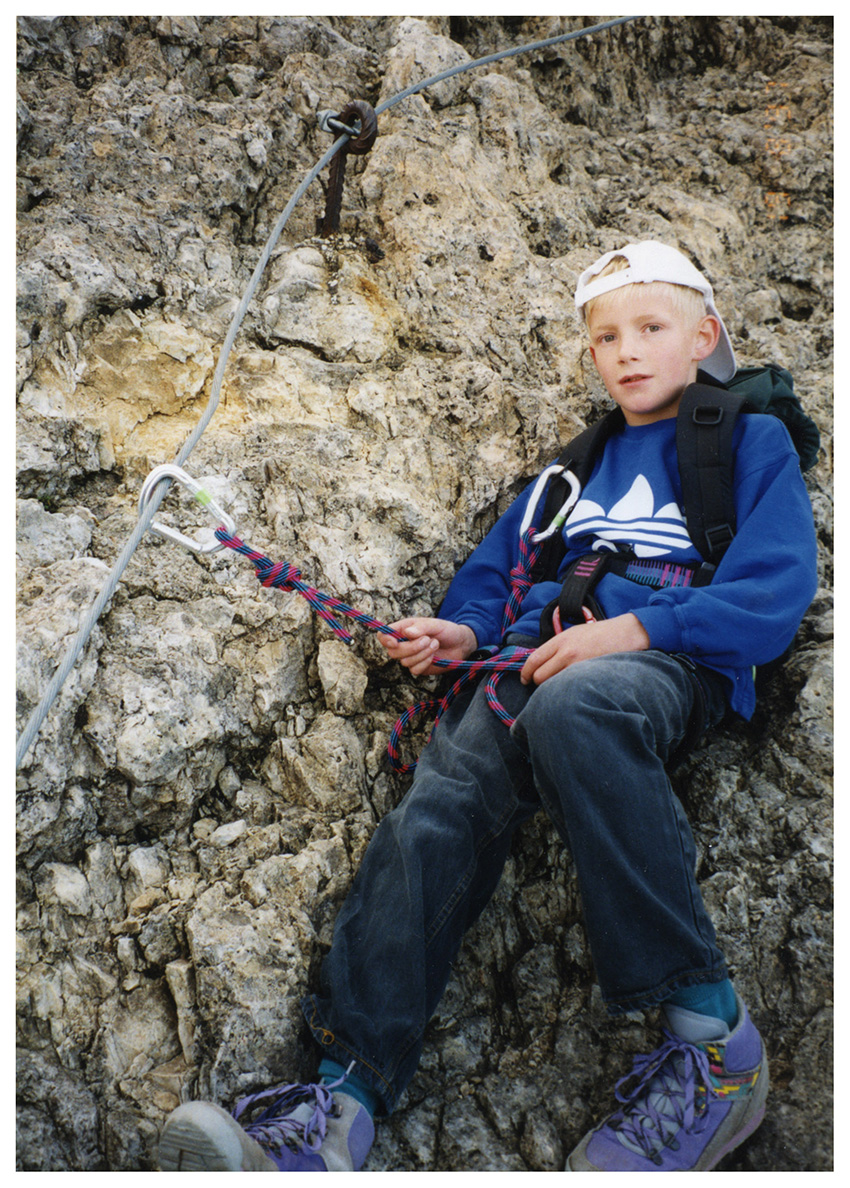
\includegraphics[angle=7,width=\textwidth]{include/images/1997.jpg}
	\end{subfigure}
	\hspace*{\fill}
	\begin{subfigure}[t]{0.49\columnwidth}
		\centering
		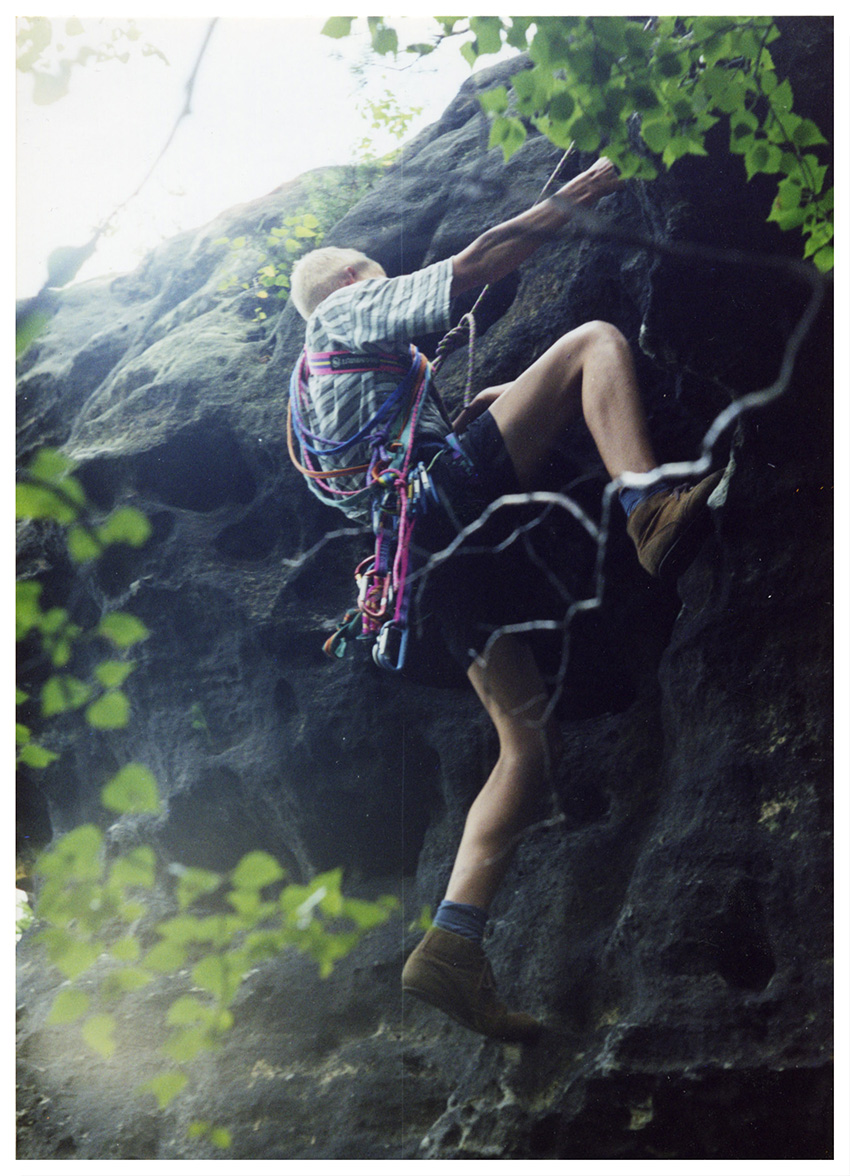
\includegraphics[angle=-5,width=\textwidth]{include/images/2002.jpg}
	\end{subfigure}
\end{figure}
\end{frame}

\begin{frame}{Eigene Forschungsprojekte -- Imagery in Sport Climbing}
\begin{figure}[h]
	\centering
	\begin{subfigure}[t]{0.49\columnwidth}
		\centering
		\begin{overpic}[width=\textwidth]{include/images/Google-Glass.jpg}
			\rbox{-1}{1}{\textcolor{source}{\tiny{Quelle: \href{https://de.wikipedia.org/wiki/Datei:Google_Glass_Main.jpg}{Wikipedia}}}}
		\end{overpic}
		\label{fig:google-glass}
	\end{subfigure}
	\hspace*{\fill}
	\begin{subfigure}[t]{0.49\columnwidth}
		\centering
		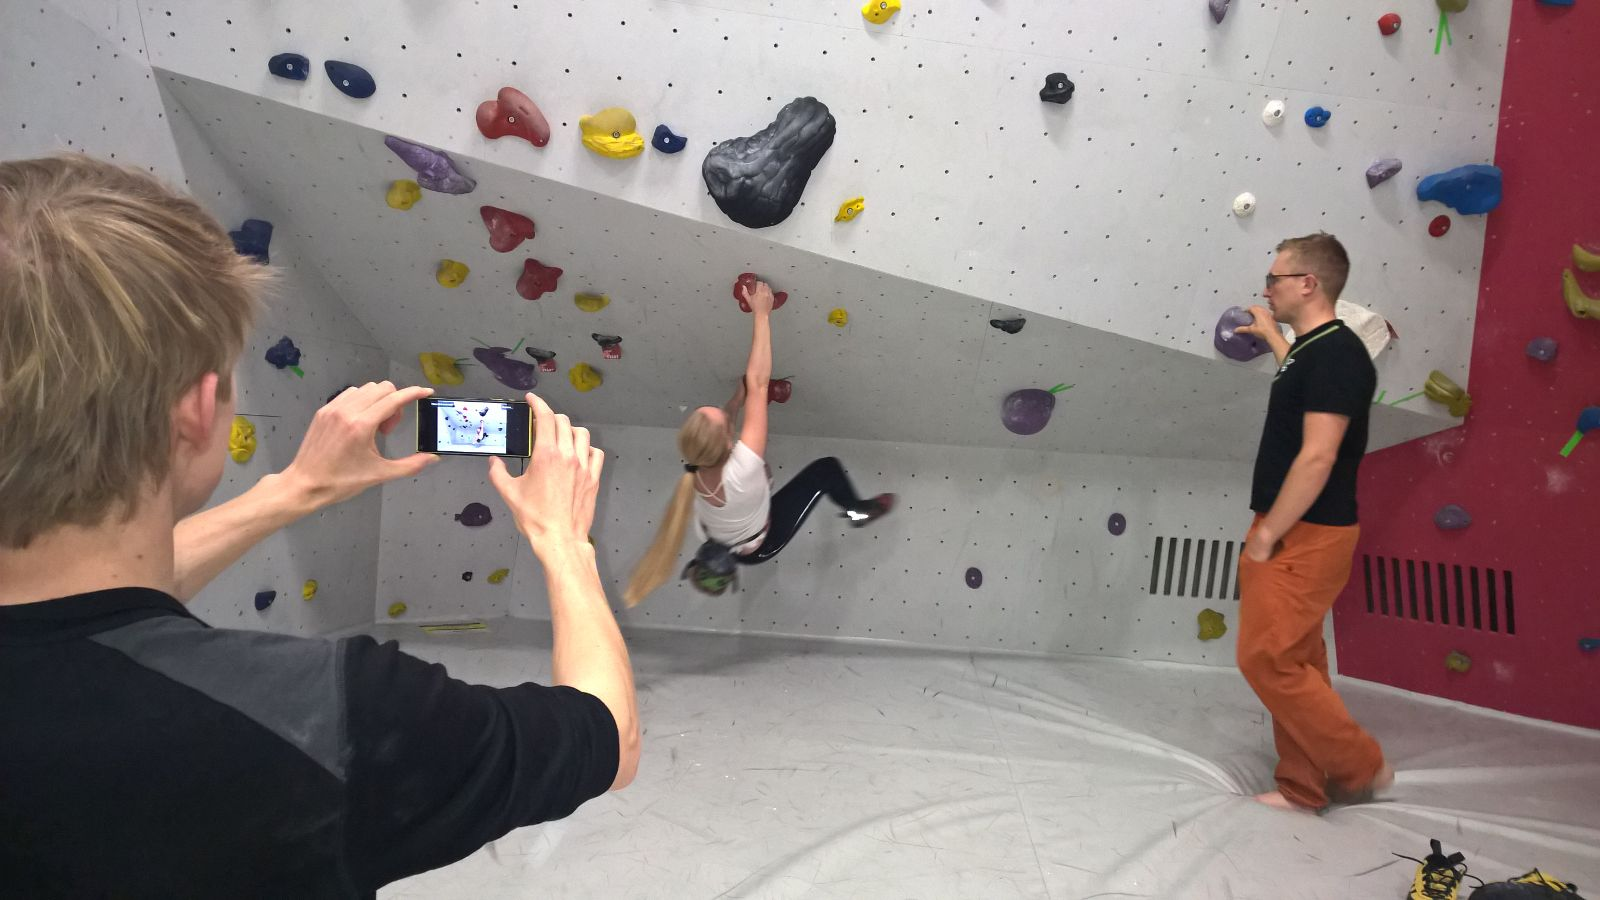
\includegraphics[width=\textwidth]{include/images/Live-Video.jpg}
		\label{fig:live-video-action}
	\end{subfigure}
	\caption{Livebildübertragung vom Smartphone (Kamera) an Google Glass Brille (Display). \\Die Kletterin kann sich selbst beim Klettern sehen, während sie klettert.}
	\label{fig:live-video}
\end{figure}
\end{frame}

\begin{frame}{Eigene Forschungsprojekte -- Crimp\textcolor{tertiary}{Bit}}
\begin{figure}[h]
	\centering
	\begin{subfigure}[t]{0.35\columnwidth}
		\centering
		\begin{overpic}[width=\textwidth]{include/images/myo-armband.jpg}
			\rbox{-9}{1}{\textcolor{source}{\tiny{Quelle: \href{https://www.myo.com}{Thalmic Labs Inc.}}}}
		\end{overpic}
		\label{fig:myo-armband}
	\end{subfigure}
	\hspace*{\fill}
	\begin{subfigure}[t]{0.62\columnwidth}
		\centering
		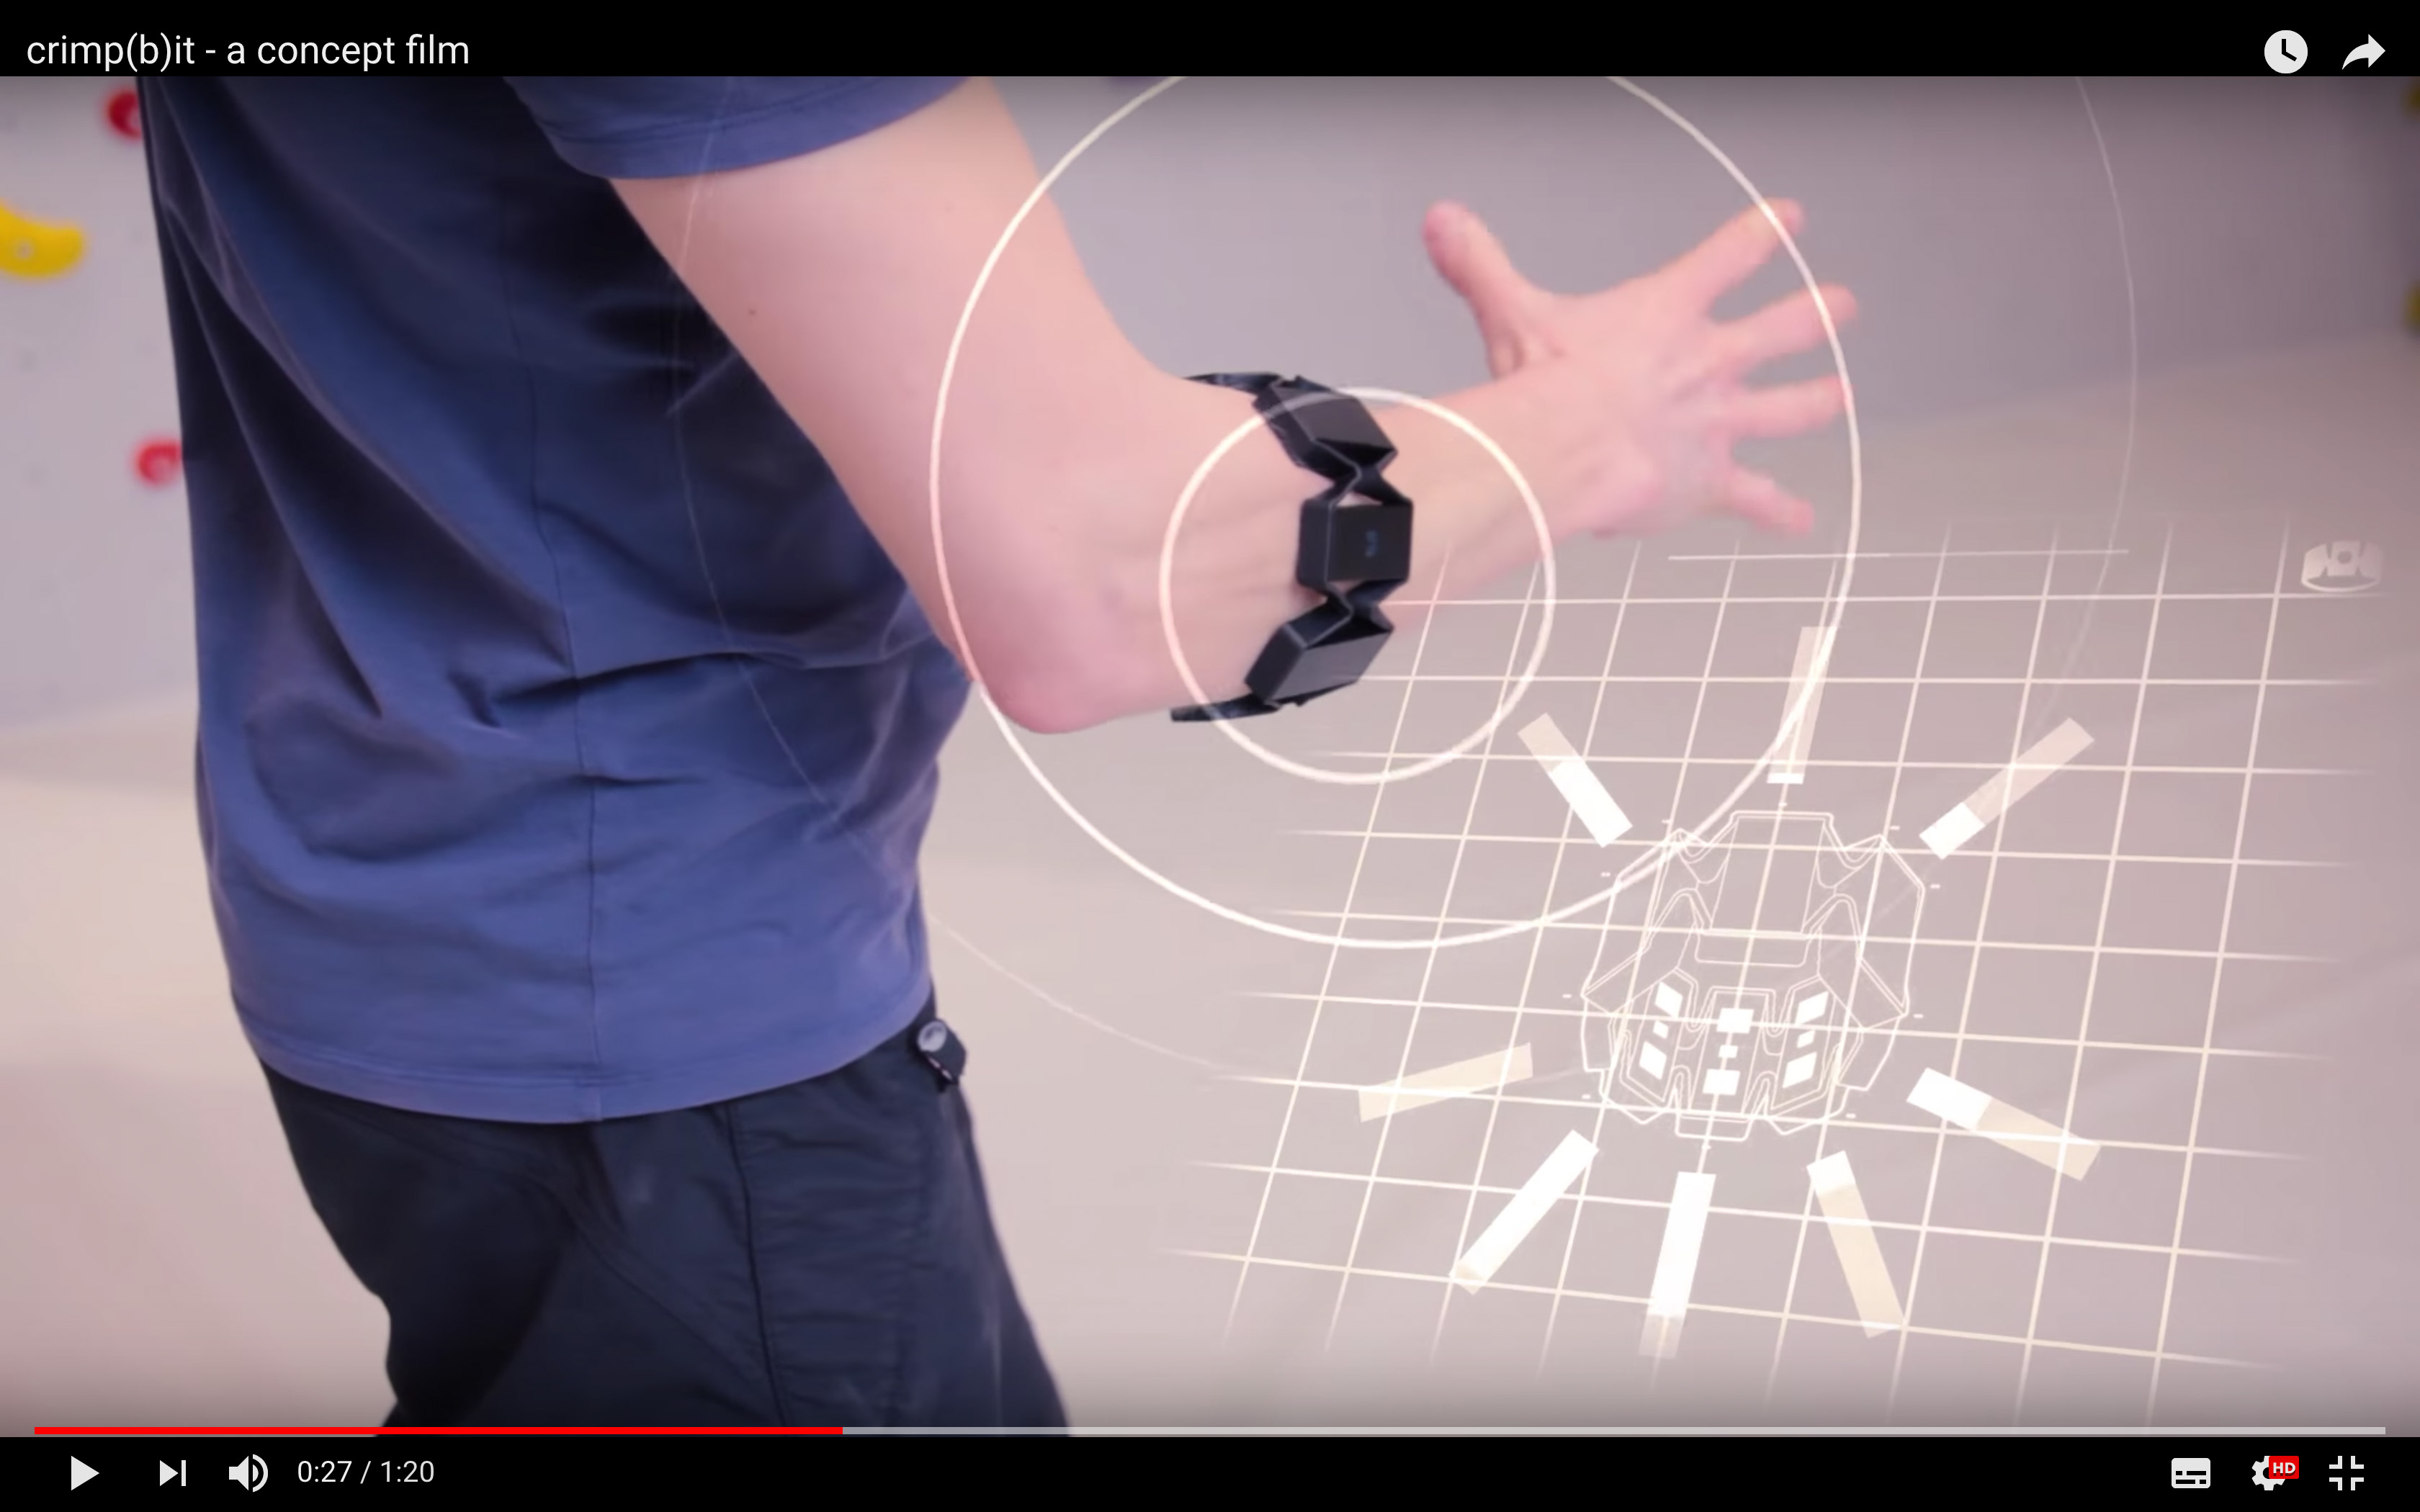
\includegraphics[width=\textwidth]{include/images/myo-demo.jpg}
		\label{fig:crimpbit-demo}
	\end{subfigure}
	\caption{MYO Armband zur Gestenerkennung als Sensor für potentiell schädliche Greifbewegungen.}
	\label{fig:crimpbit}
\end{figure}
\end{frame}

{
\usebackgroundtemplate{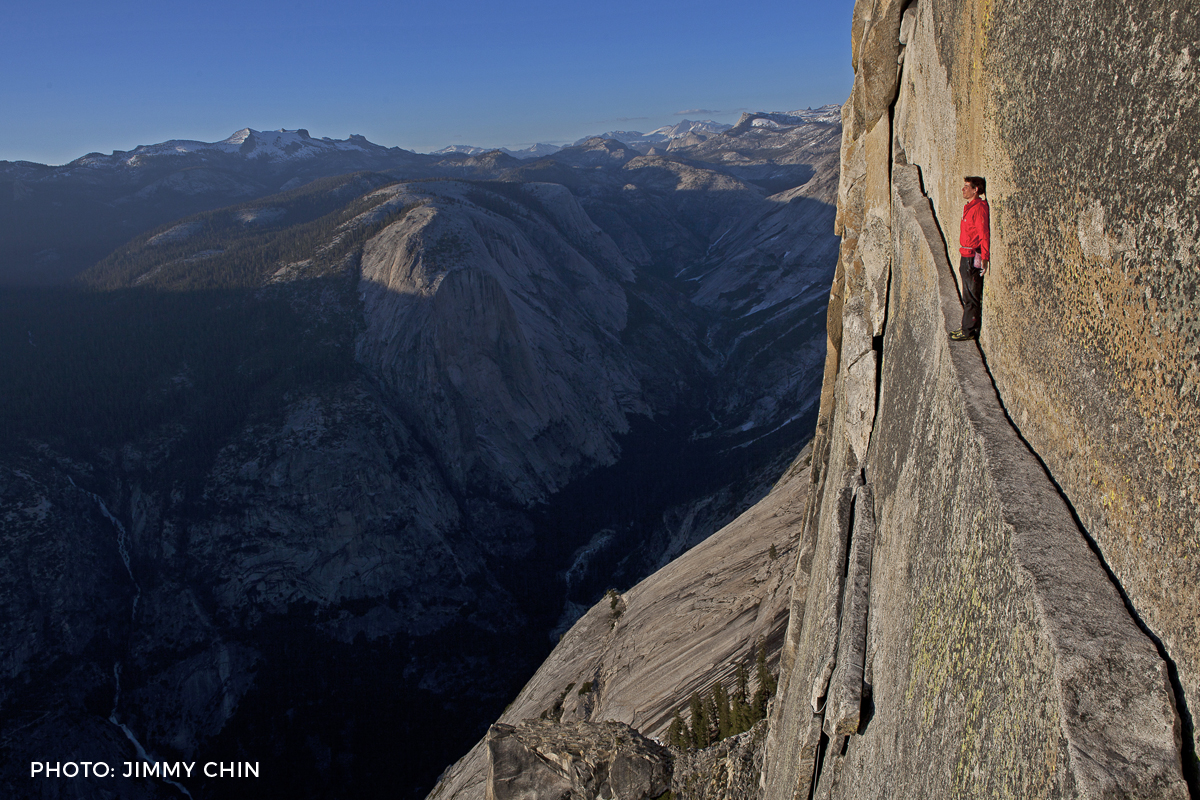
\includegraphics[width=\paperwidth]{include/images/honnold.jpg}}
\begin{frame}{Höhenangst \textcolor{gray}{\&} \textcolor{tertiary}{Sturzangst}}
\begin{textblock}{140}(5,83)
	\textcolor{tertiary}{\textcopyright Jimmy Chin}
	\href{http://www.accidentofgeography.com/alex-honnold-epic-el-capitan-triumph/}{www.accidentofgeography.com} 
\end{textblock}
\end{frame}
}

{
	\usebackgroundtemplate{\movie[label=clip-1,width=\paperwidth,height=\paperheight,open,once,showcontrols=false]{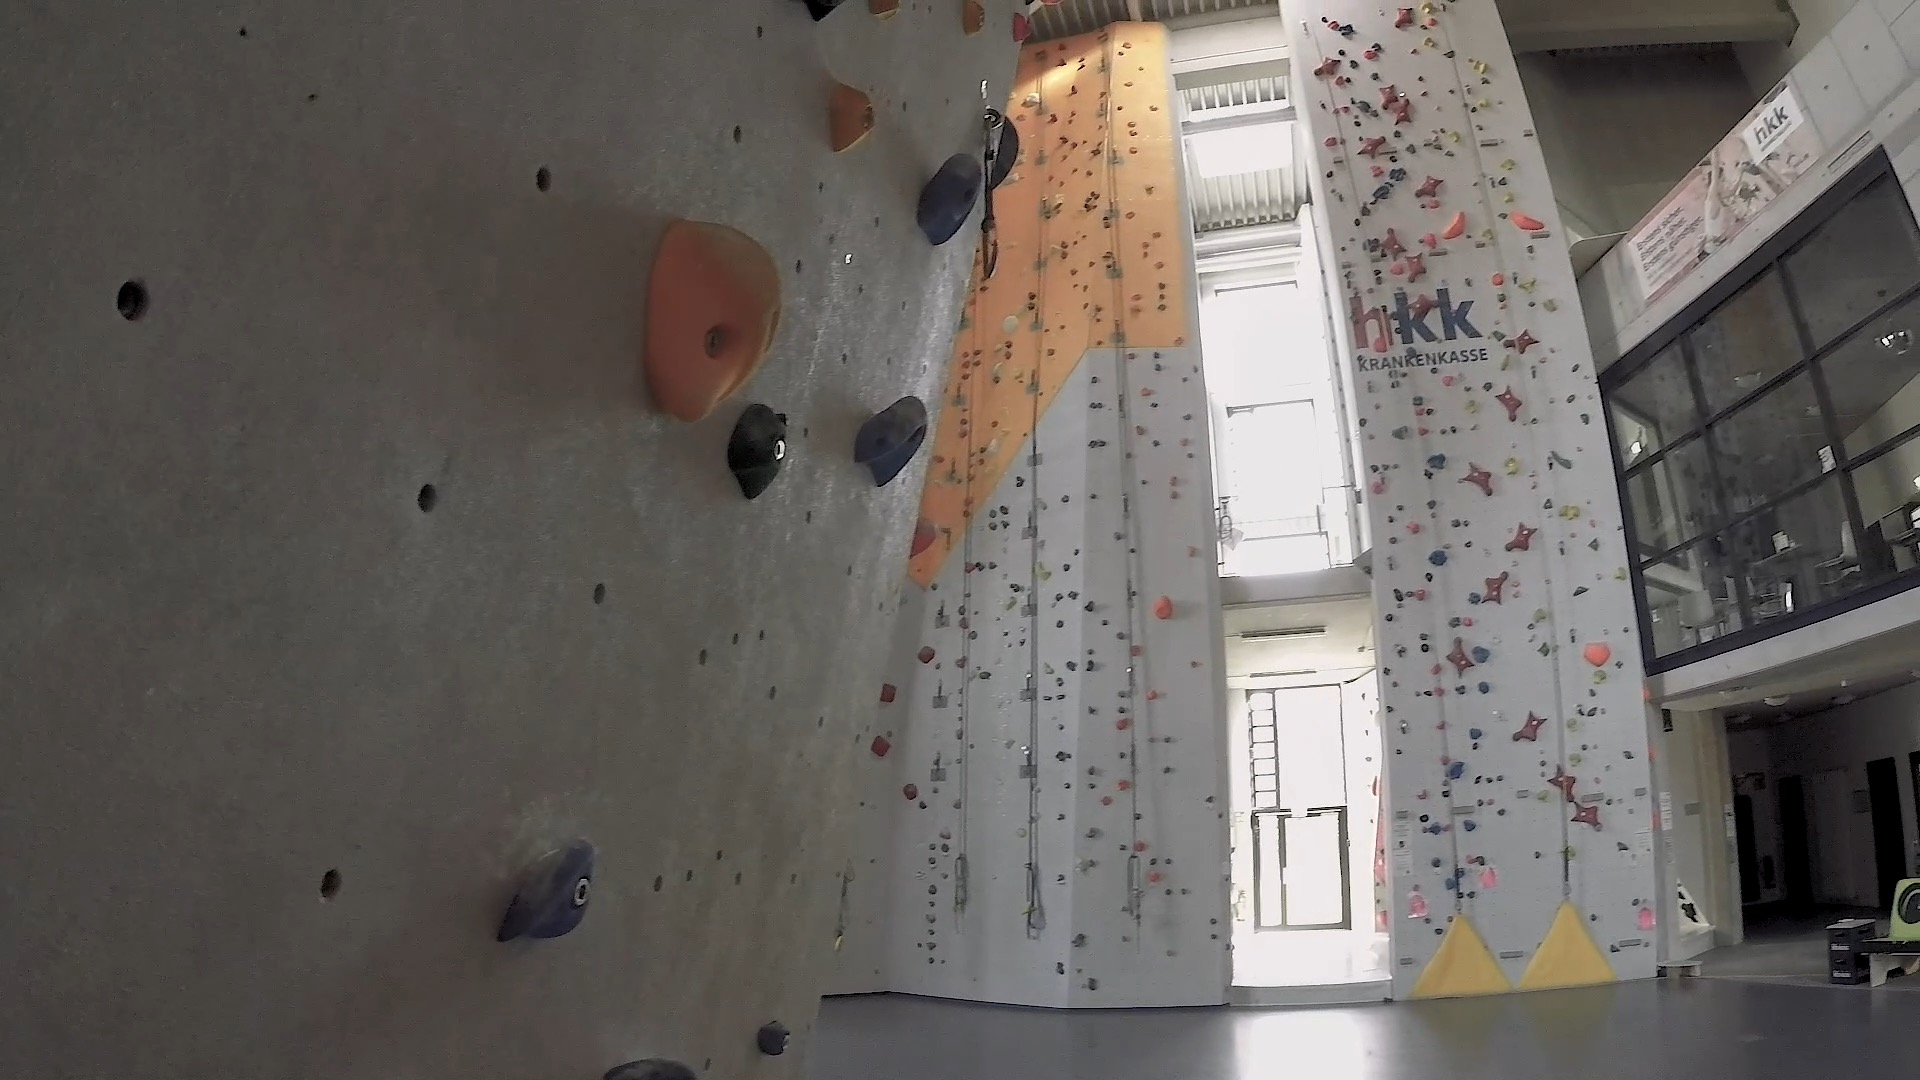
\includegraphics[width=\paperwidth]{include/images/master-thesis-clip-1.jpg}}{include/videos/master-thesis-clip-1.mov}}
	\begin{frame}[standout]
	\end{frame}
}

\begin{frame}{Lässt sich \textcolor{tertiary}{Sturzangst}, wie auch Höhenangst, \textcolor{tertiary}{in VR} auslösen?}
	\centering
	\begin{overpic}[height=0.8\textheight]{include/images/samsung-gear-acrophobia-original.jpg}
		\rbox{-4}{1}{\textcolor{source}{\tiny{Quelle: \href{https://vrscout.com/projects/fear-of-heights-samsung-gear-vr/}{VRscout}}}}
	\end{overpic}
\end{frame}

\begin{frame}{Related Work mit \textcolor{tertiary}{Höhen} und \textcolor{tertiary}{Kanten}}
\begin{columns}
	\begin{column}{0.45\textwidth}
		\begin{center}
			\begin{overpic}[height=0.8\textheight]{include/images/pijpers.jpg}
				\rbox{-15}{1}{\textcolor{black}{\tiny{Quelle: \href{https://www.researchgate.net/figure/Side-view-of-the-virtual-environment-Subjects-start-in-the-Training-Room-and-later-enter_fig1_247181822}{ResearchGate}}}}
			\end{overpic}
		\end{center}
	\end{column}
	\begin{column}{0.55\textwidth}
		\begin{center}
			\begin{overpic}[height=0.8\textheight]{include/images/meehan.jpg}
				\rbox{-1}{1}{\textcolor{source}{\tiny{Quelle: \href{https://www.researchgate.net/figure/View-of-the-20-in-pit-from-the-wooden-ledge_fig3_7596875}{ResearchGate}}}}
			\end{overpic}
		\end{center}
	\end{column}
\end{columns}
\end{frame}

{
	\usebackgroundtemplate{\movie[label=clip-1,width=\paperwidth,height=\paperheight,open,once,showcontrols=false]{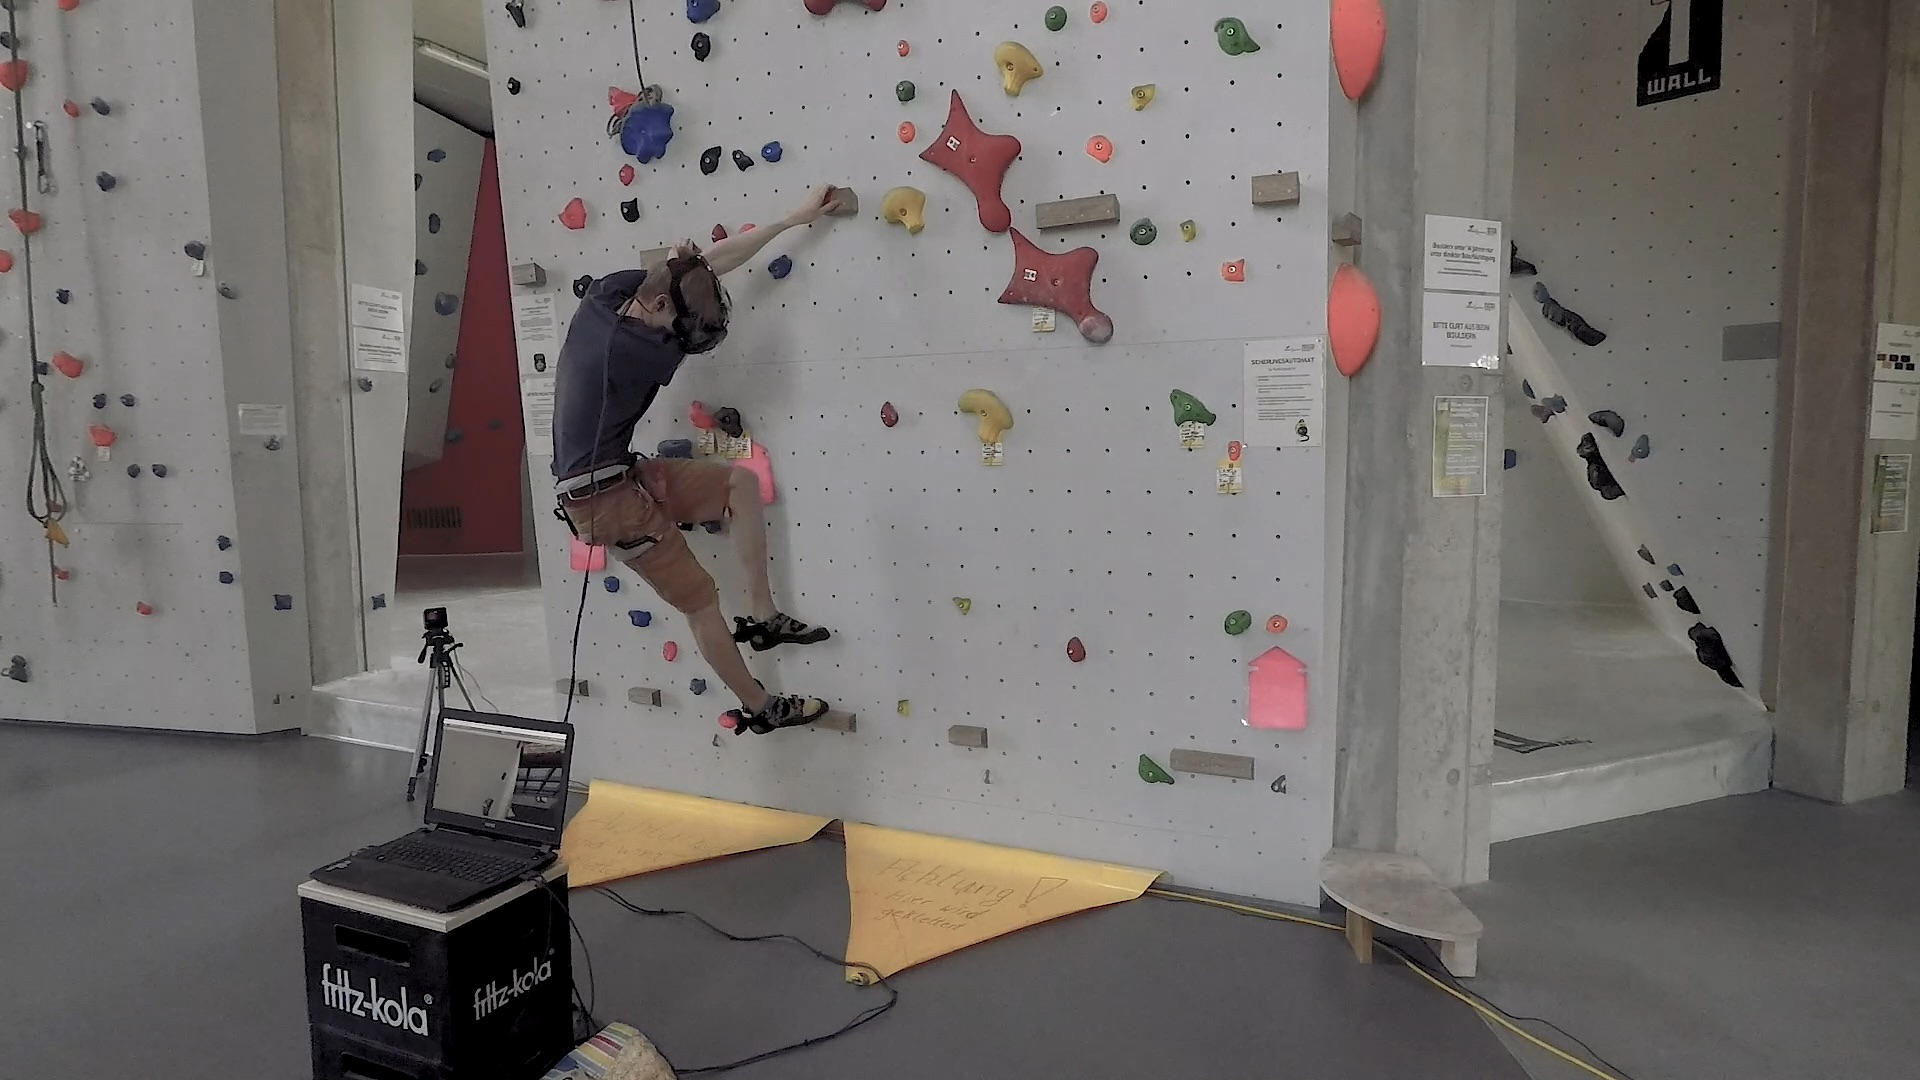
\includegraphics[width=\paperwidth]{include/images/master-thesis-clip-2.jpg}}{include/videos/master-thesis-clip-2.mov}}
	\begin{frame}[standout]
	\end{frame}
}

{
	\usebackgroundtemplate{\movie[label=clip-1,width=\paperwidth,height=\paperheight,open,once,showcontrols=false]{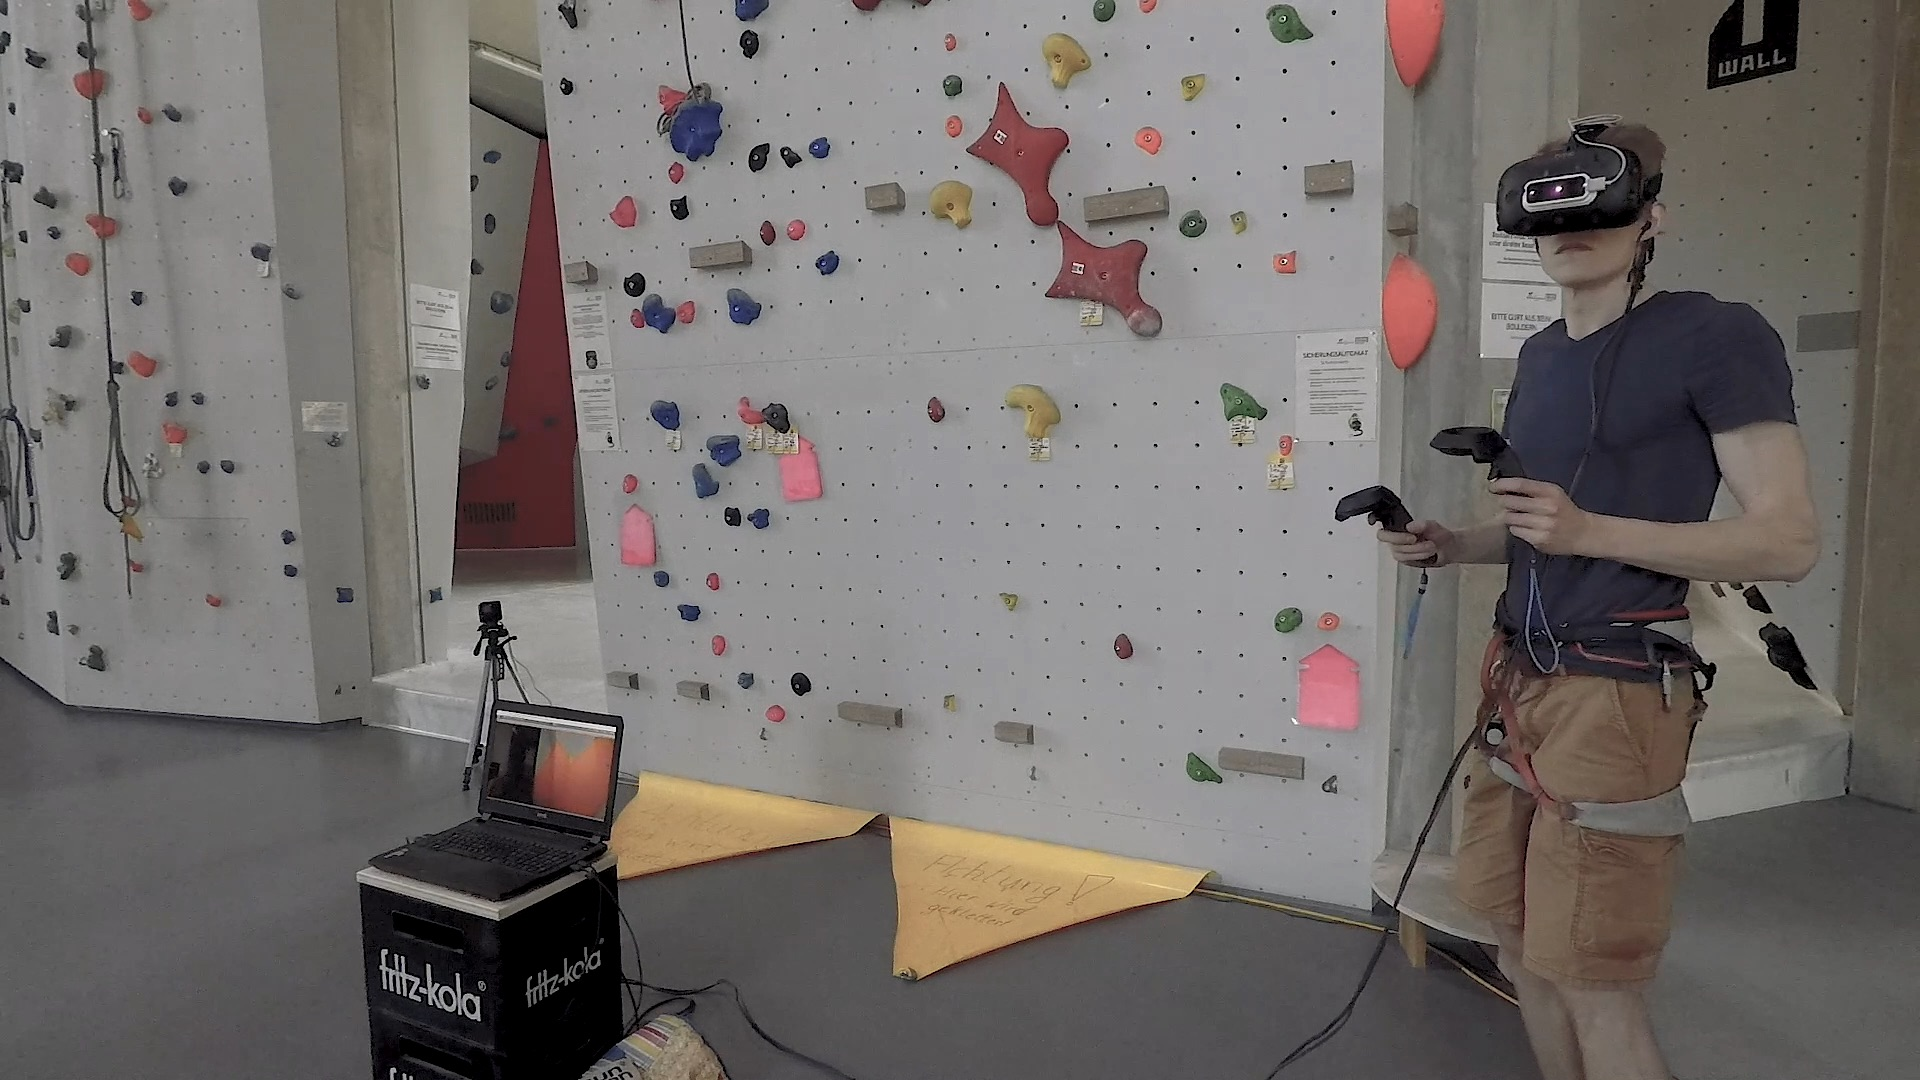
\includegraphics[width=\paperwidth]{include/images/master-thesis-clip-3.jpg}}{include/videos/master-thesis-clip-3.mov}}
	\begin{frame}[standout]
	\end{frame}
}

\section{Studie}

\begin{frame}{Versuchsbedingungen}
\begin{columns}
	\begin{column}{0.5\textwidth}
		\begin{enumerate}[label=\textbf\textcolor{tertiary}{\Alph*}]
			\item Reales Klettern an Griffen und Tritten
			\\\textcolor{source}{\SI{10}{\meter} über Grund}
			\item Klettern in \gls{VR} an Griffen und Tritten
			\\\textcolor{source}{visuell \SI{10}{\meter} über Grund}
			\item Klettern in \gls{VR} mit Game Controllern
			\\\textcolor{source}{visuell \SI{10}{\meter} über Grund}
		\end{enumerate}
	\end{column}
	\begin{column}{0.5\textwidth}
		\begin{center}
			\vspace*{-15mm}
			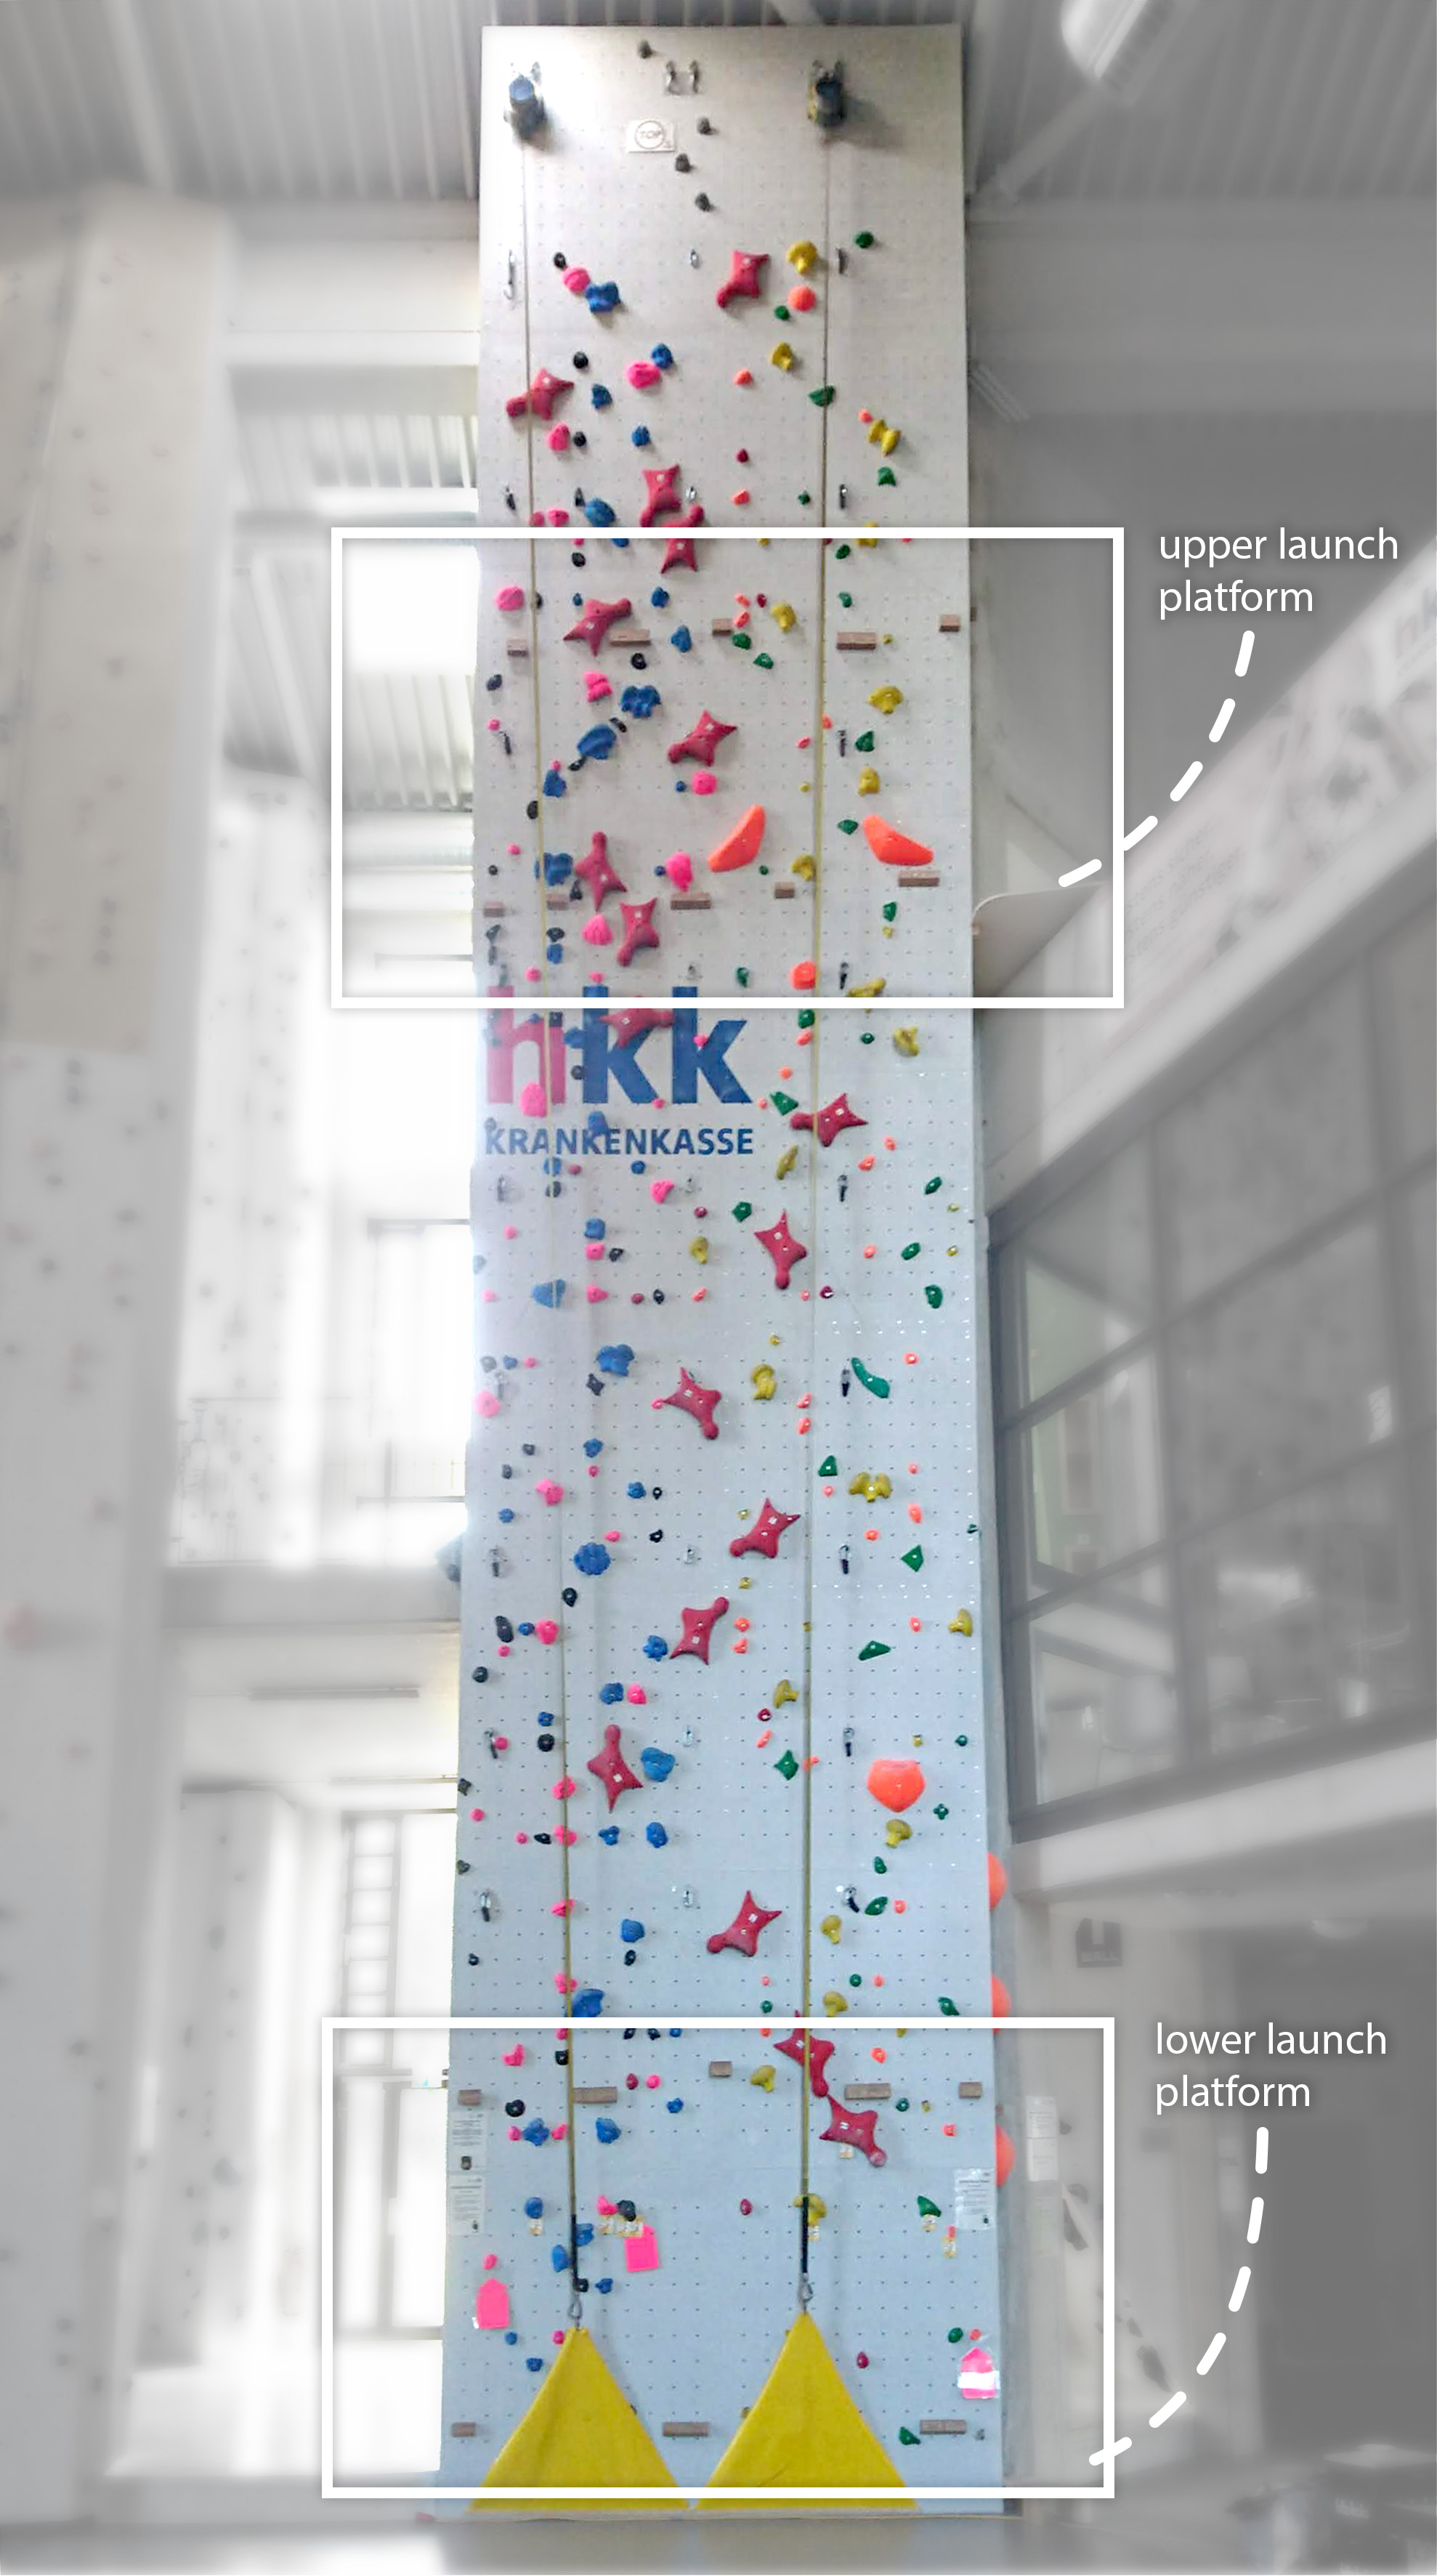
\includegraphics[height=1.2\textheight]{include/images/climbing-wall-photo.jpg}
		\end{center}
	\end{column}
\end{columns}
\end{frame}

\subsection{Technische Umsetzung}

\begin{frame}{\currentname{} -- Virtual Reality System}
	\begin{figure}
		\begin{subfigure}[t]{0.49\textwidth}
			\centering
			\begin{overpic}[width=\textwidth]{include/images/vive-kit.jpg}
				\rbox{-1}{1}{\textcolor{source}{\tiny{Quelle: \href{			https://www.inet.se/produkt/x107651/htc-vive}{HTC Corporation}}}}
			\end{overpic}
			\caption{HTC VIVE + Basistation + Controller}
		\end{subfigure}
		\begin{subfigure}[t]{0.49\textwidth}
			\centering
			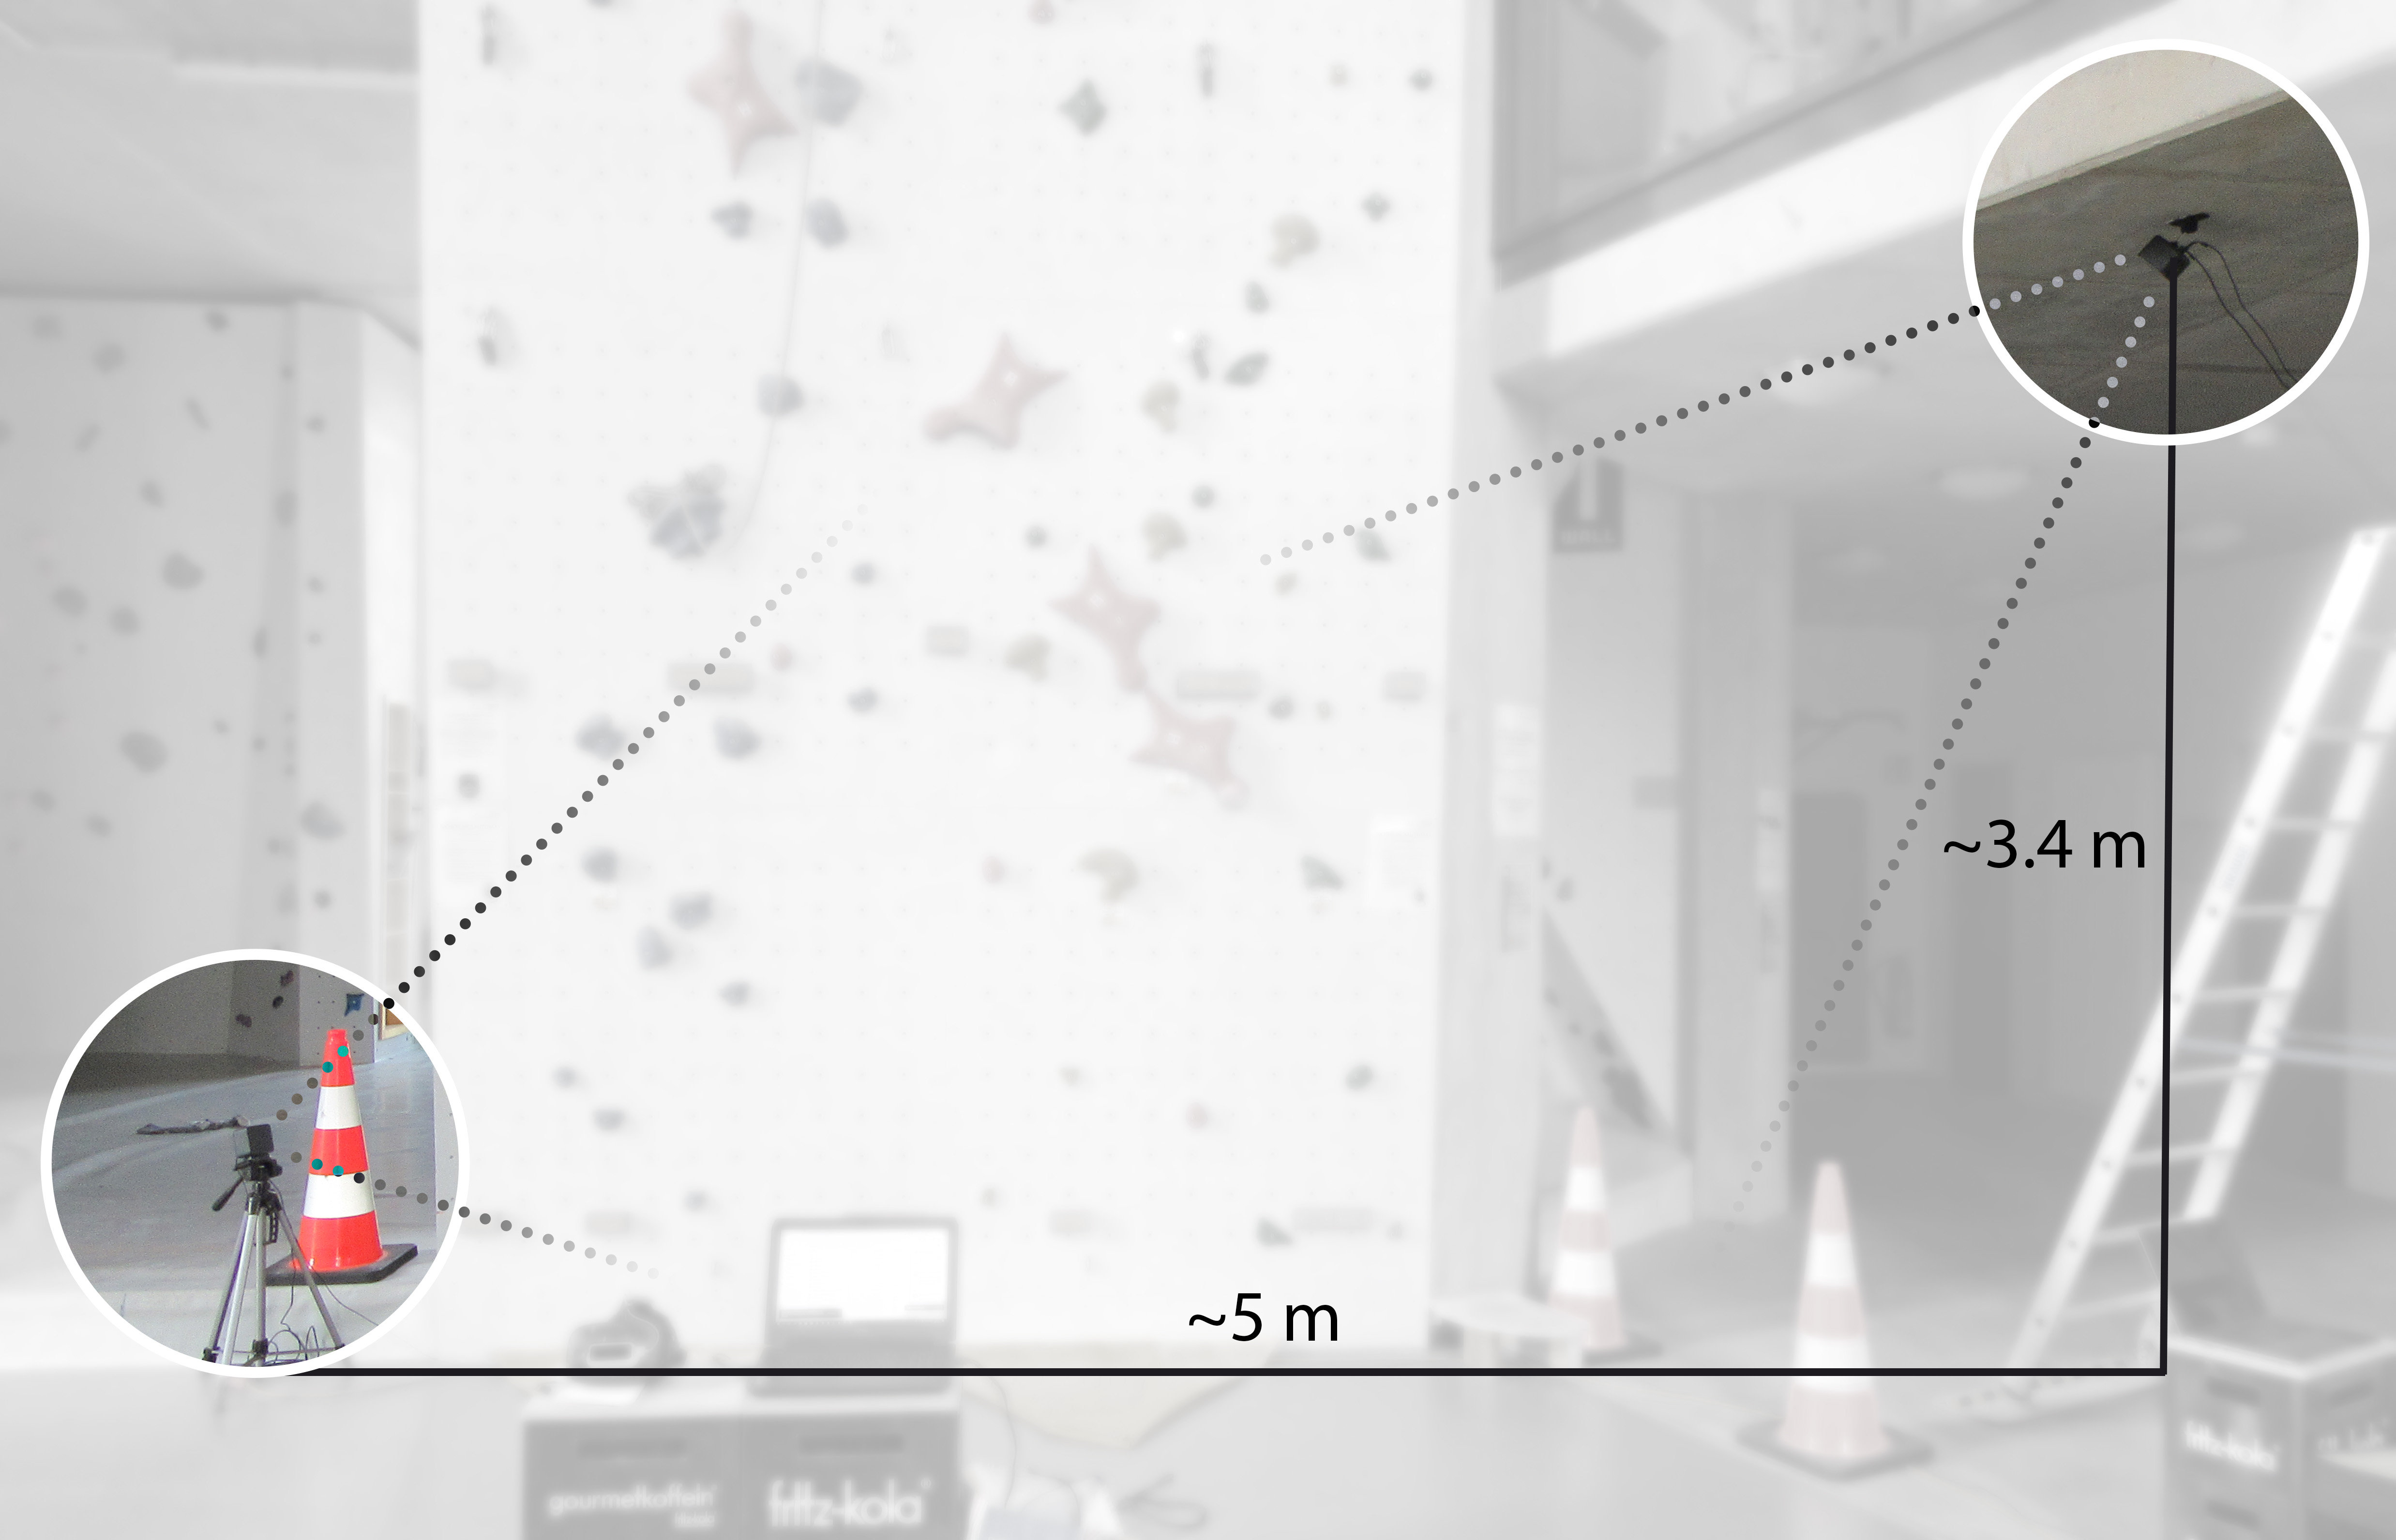
\includegraphics[width=\textwidth]{include/images/vive-setup-solution.jpg}
			\caption{HTC VIVE Position der Basistationen}
		\end{subfigure}
	\end{figure}
\end{frame}

\begin{frame}{\currentname{} -- Fuß Tracking}
\begin{figure}
	\centering
	\begin{subfigure}[t]{0.49\textwidth}
		\centering
		\includegraphics[width=\textwidth]{include/images/foot-tracking-tracker.png}
		\caption{VIVE Tracker befestigt an der Ferse}
		\label{fig:foot-tracking-tracker}
	\end{subfigure}
	\hfill
	\begin{subfigure}[t]{0.49\textwidth}  
		\centering 
		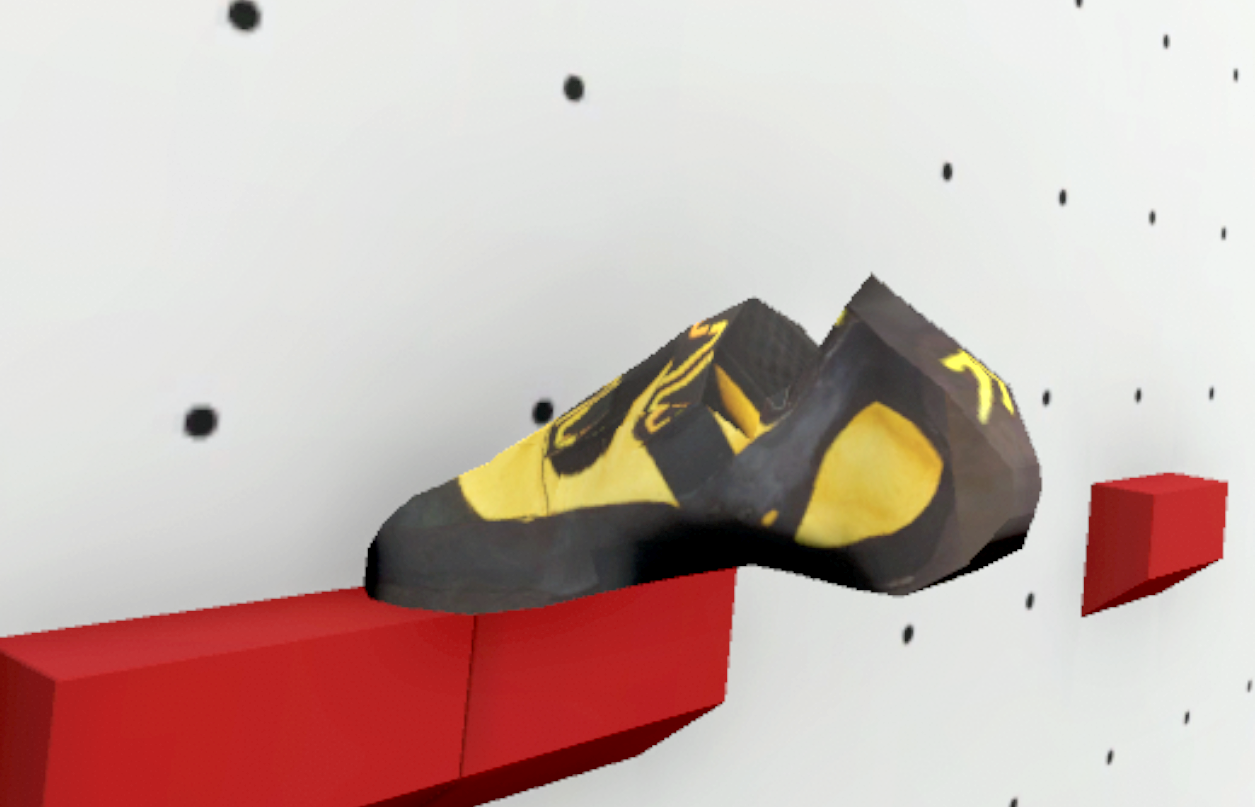
\includegraphics[width=\textwidth]{include/images/foot-tracking-result.png}
		\caption{Übertragenes Tracking auf 3D Modell in Unity}
		\label{fig:foot-tracking-result}
	\end{subfigure}
	\label{fig:foot-tracking}
\end{figure}
\end{frame}

\begin{frame}{\currentname{} -- Hand Tracking}
\begin{figure}
	\centering
	\begin{subfigure}[t]{0.32\textwidth}
		\centering
		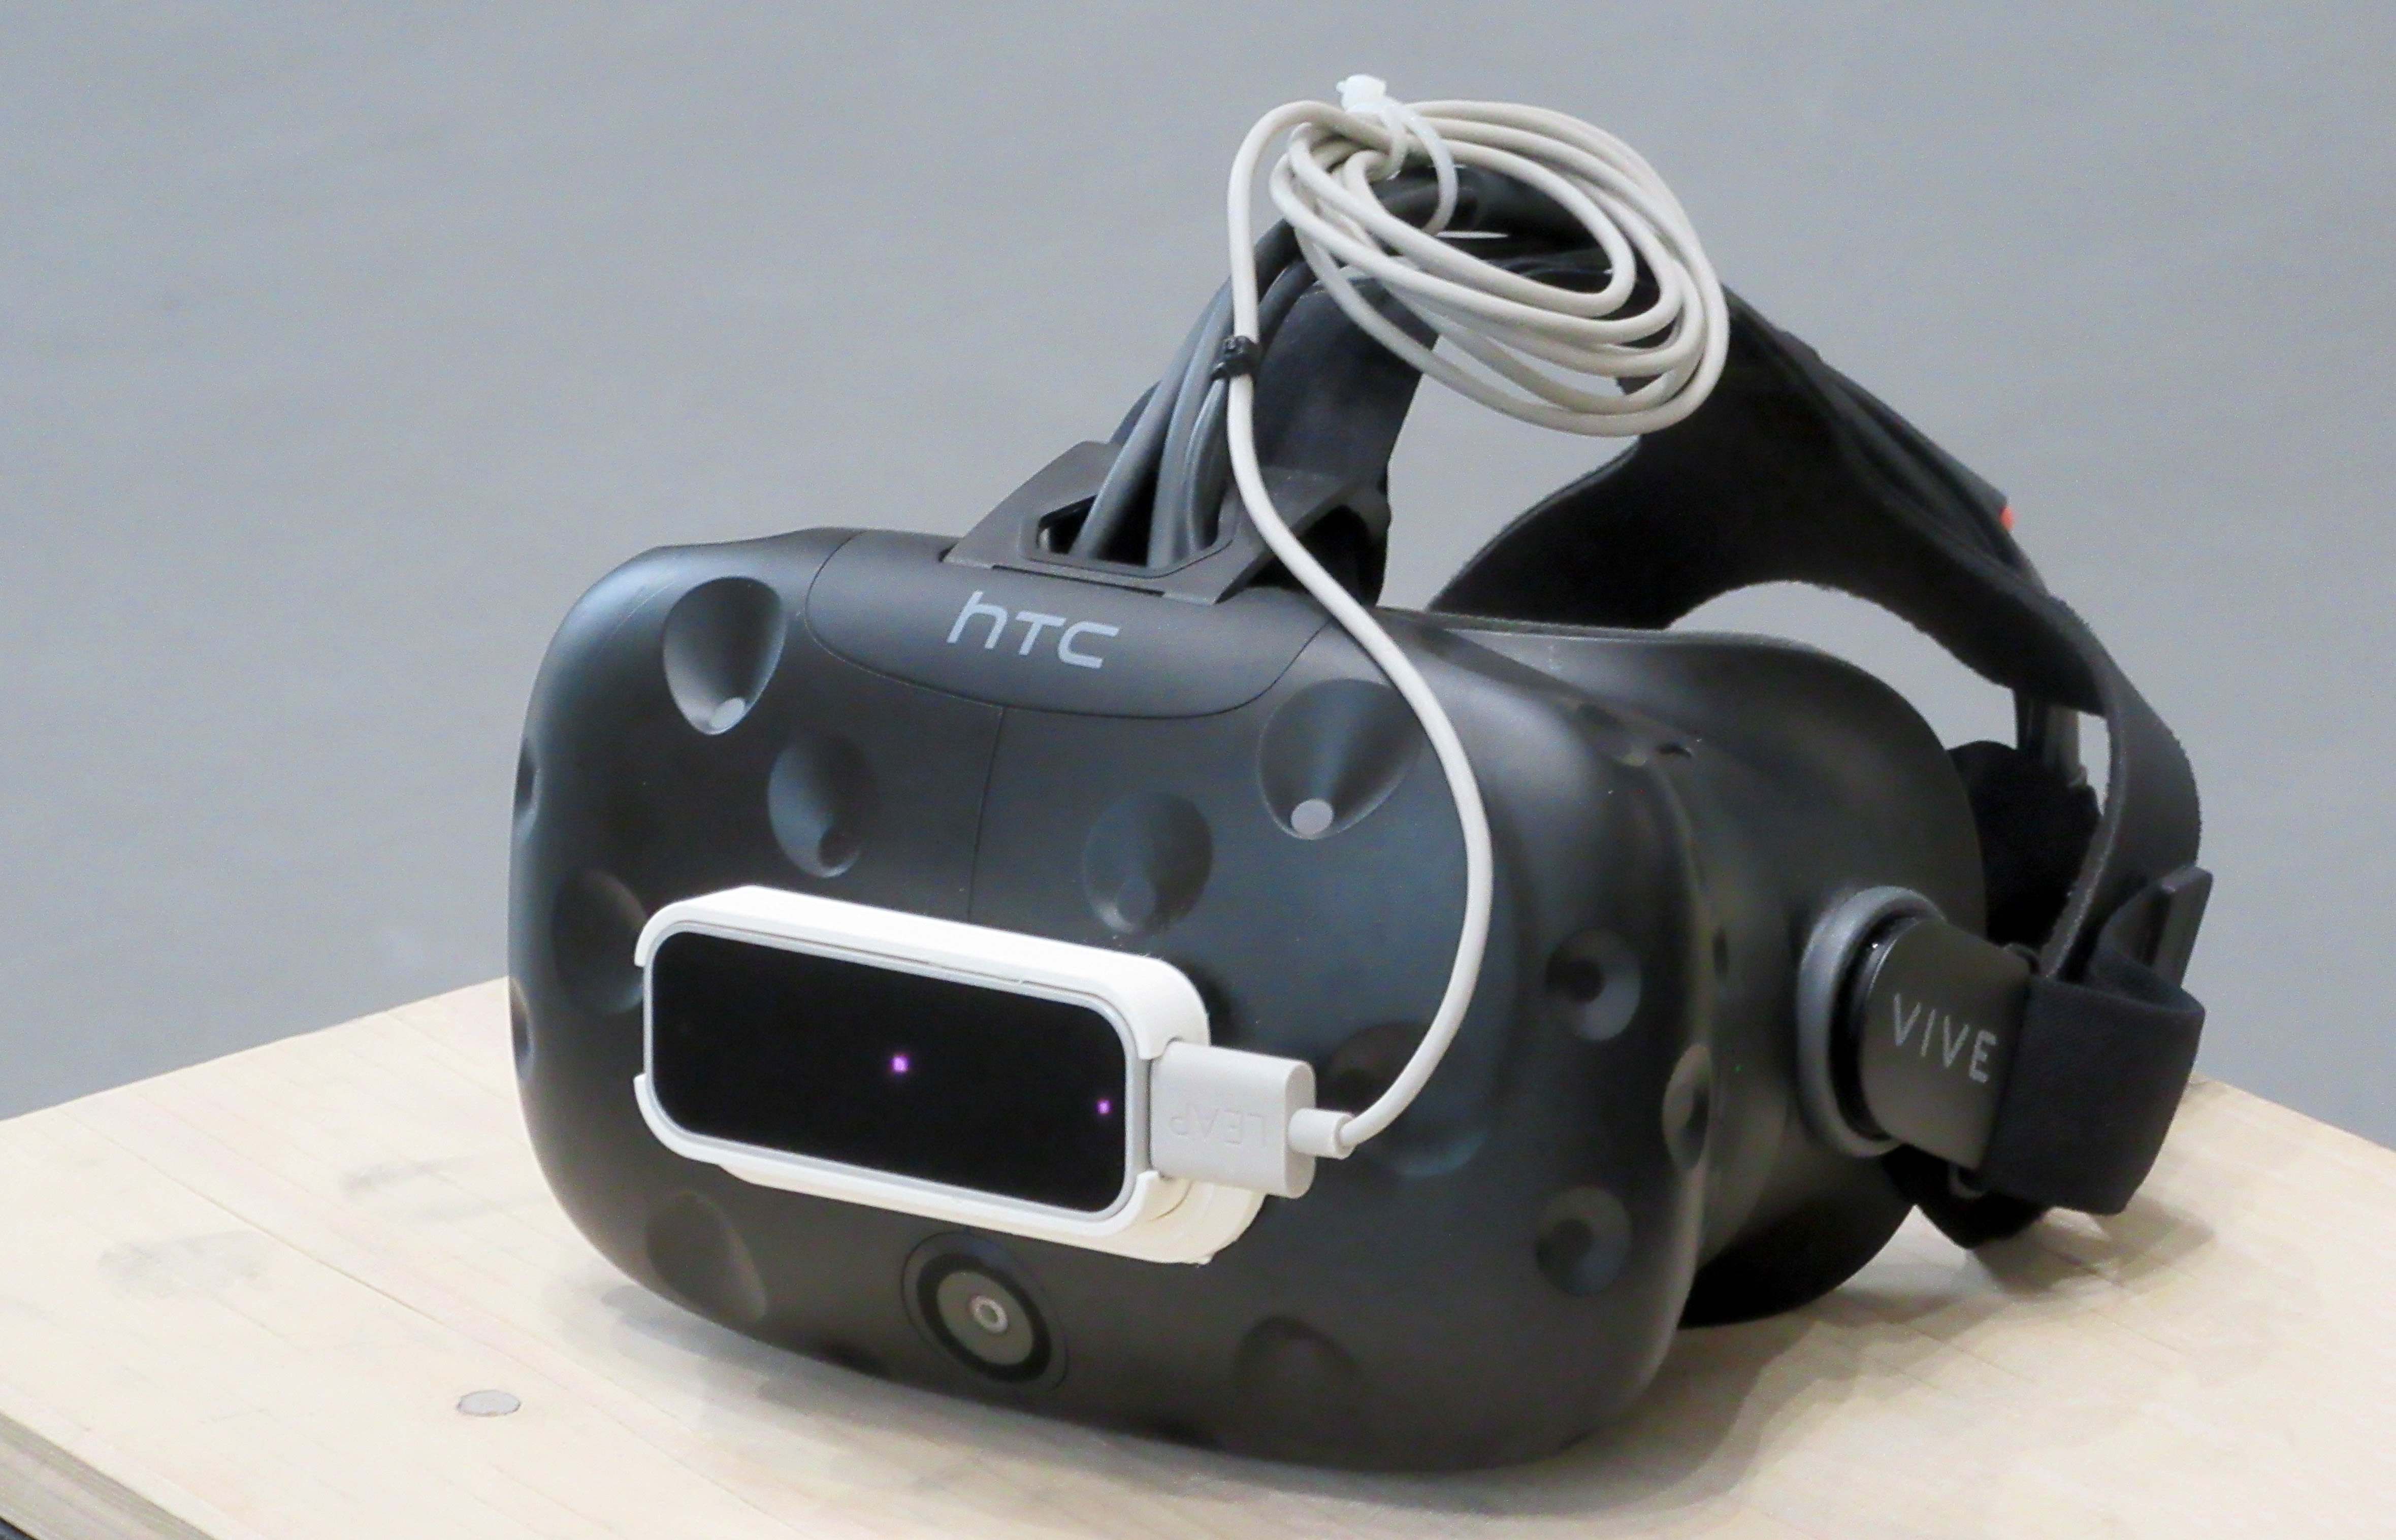
\includegraphics[width=\textwidth]{include/images/leap-motion-overlay-setup.jpg}
		\caption{LEAP Motion auf VIVE Headset}
		\label{fig:leap-motion-setup}
	\end{subfigure}
	\hfill
	\begin{subfigure}[t]{0.32\textwidth}
		\centering
		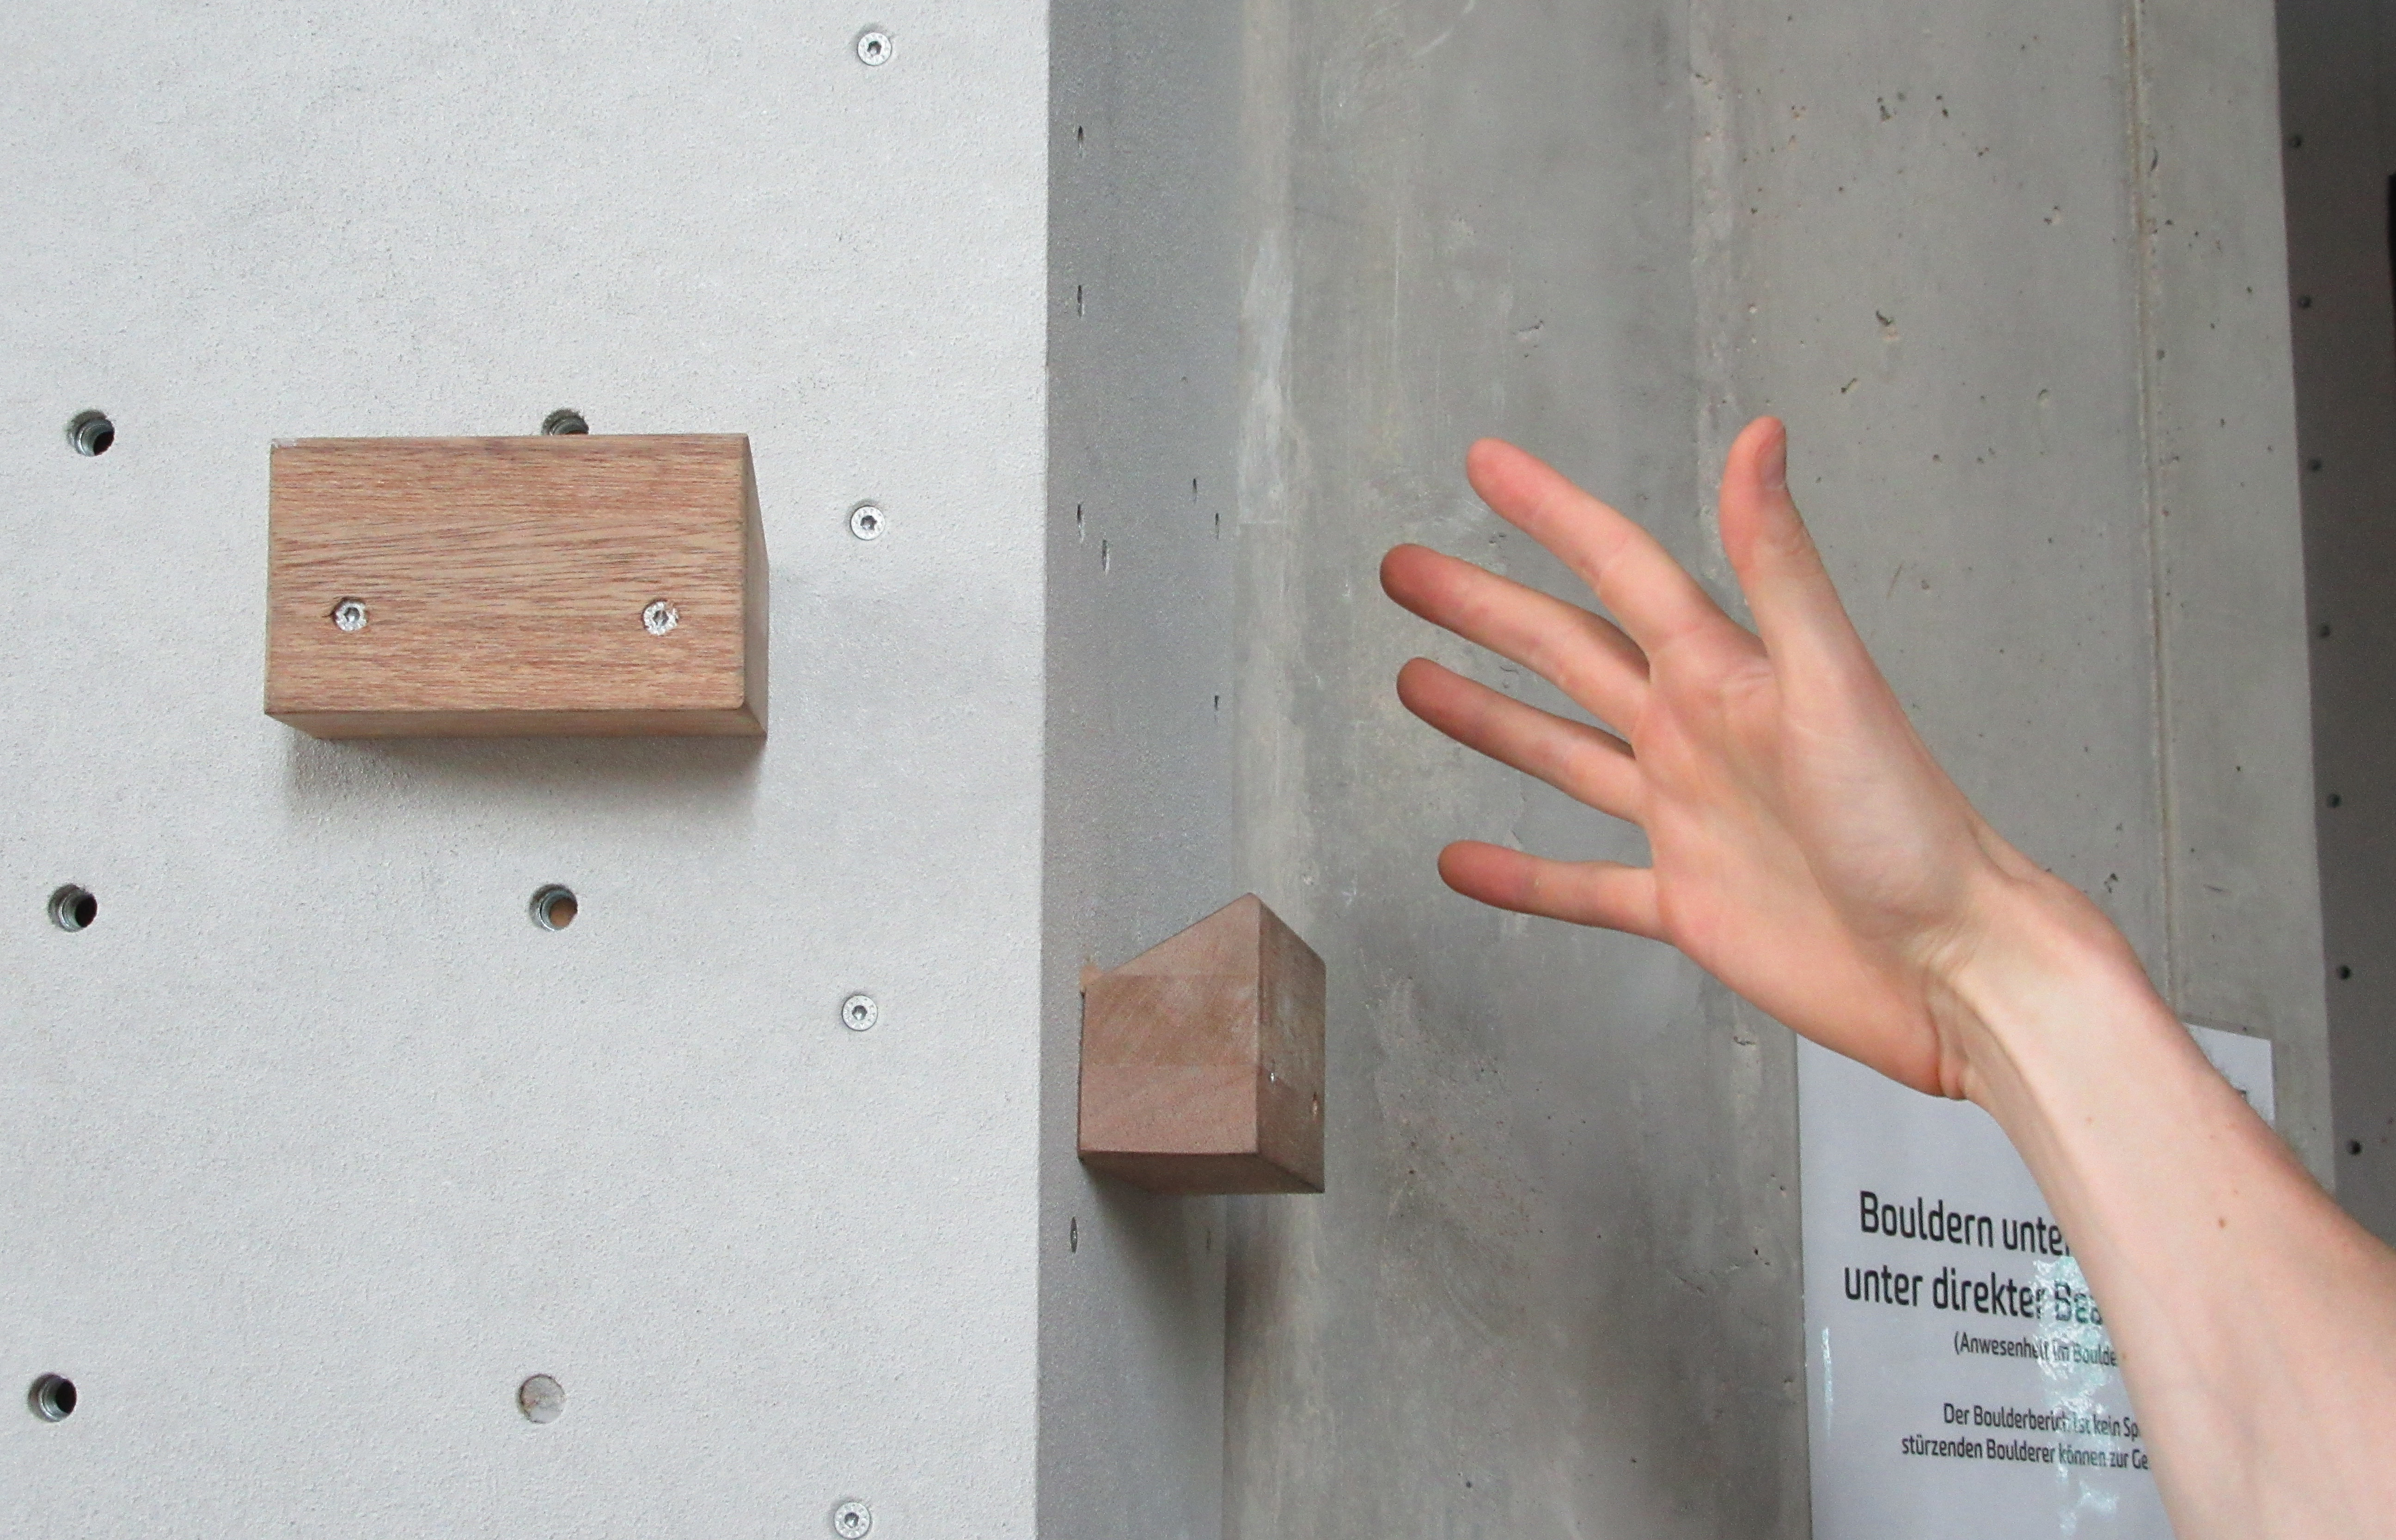
\includegraphics[width=\textwidth]{include/images/leap-motion-overlay-photo.jpg}
		\caption{Reale Perspektive (Foto)}
		\label{fig:leap-motion-overlay-photo}
	\end{subfigure}
	\hfill
	\begin{subfigure}[t]{0.32\textwidth}
		\centering
		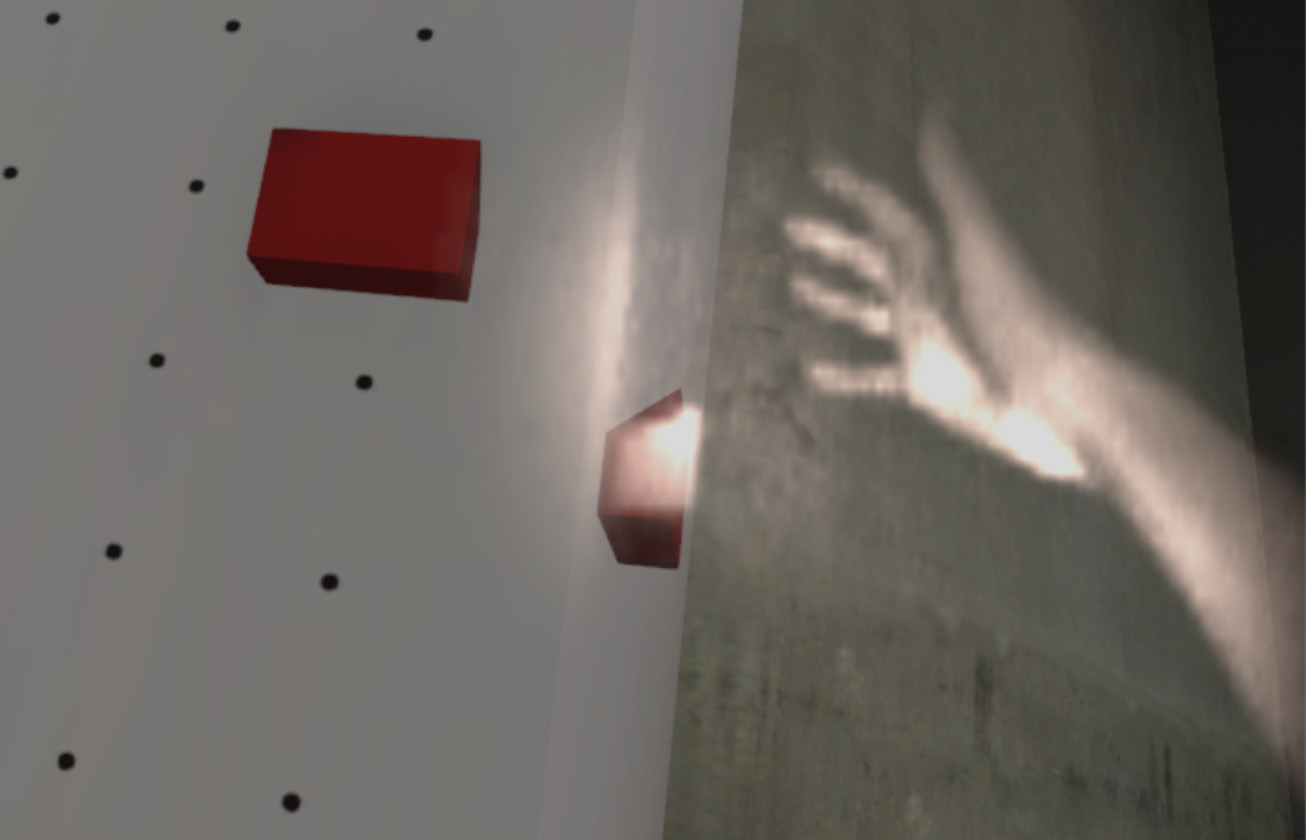
\includegraphics[width=\textwidth]{include/images/leap-motion-overlay-result.jpg}
		\caption{Resultierende des Overlays (Unity)}
		\label{fig:leap-motion-overlay-result}
	\end{subfigure}
	\captionsetup{subrefformat=parens}
	\caption[Leap Motion hand tracking]{Hand Overlay erzeugt aus einem Infrarotbild des LEAP Motion Sensors \subref{fig:leap-motion-setup} welches weich anhand des 3D Modells maskiert wird $\rightarrow$ nahegelegene Griffe bleiben sichtbar \subref{fig:leap-motion-overlay-result}}
	\label{fig:leap-motion-overlay}
\end{figure}
\end{frame}

\begin{frame}{\currentname{} -- Biosignalerfassung}
\begin{figure}
	\centering
	\begin{subfigure}[b]{0.49\textwidth}
		\centering
		{
			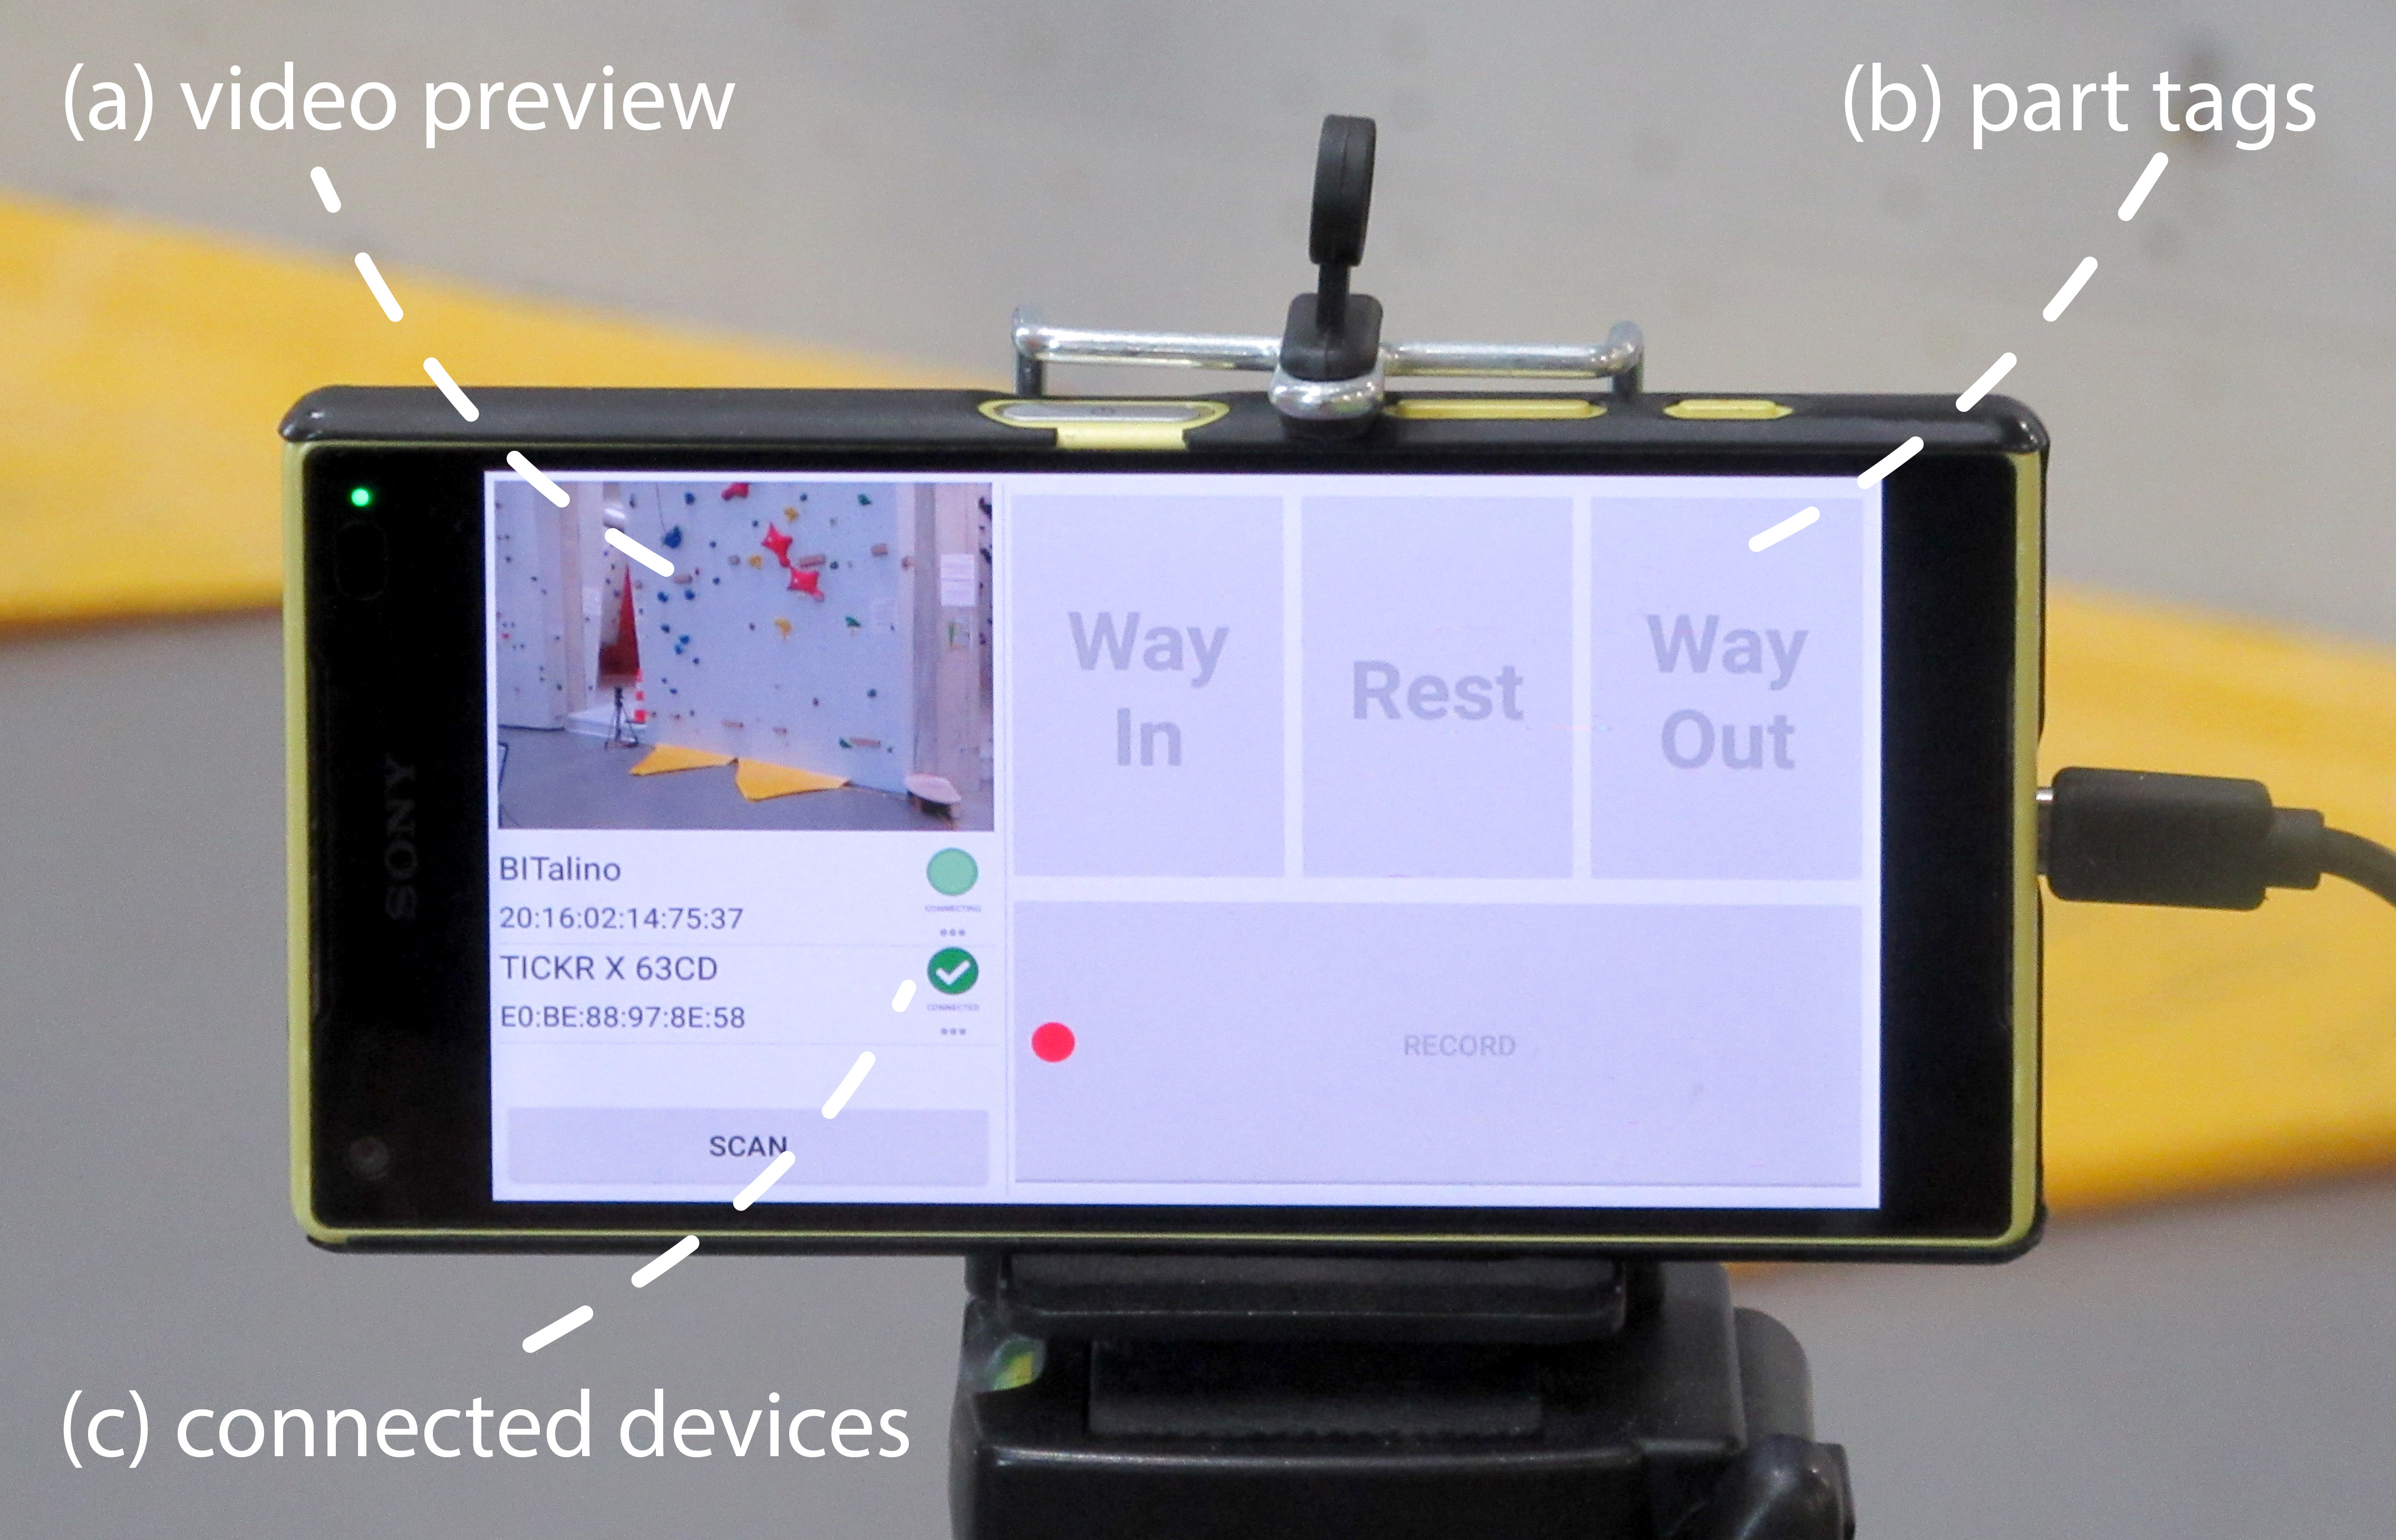
\includegraphics[width=\textwidth]{include/images/android-app-photo.jpg}
			\phantomsubcaption\label{fig:android-app-preview}
			\phantomsubcaption\label{fig:android-app-parts}
			\phantomsubcaption\label{fig:android-app-devices}
		}
		\captionsetup{subrefformat=parens}
		\caption{Android App zur Erfassung der Biosignale, mit Videovorschau \subref{fig:android-app-preview}, einer Liste verbundener Sensoren \subref{fig:android-app-devices} und Knöpfen zum Markieren der Versuchsabschnitte \subref{fig:android-app-parts}}
		\label{fig:android-app}
	\end{subfigure}
	\hfill
	\begin{subfigure}[b]{0.49\textwidth}  
		\centering
		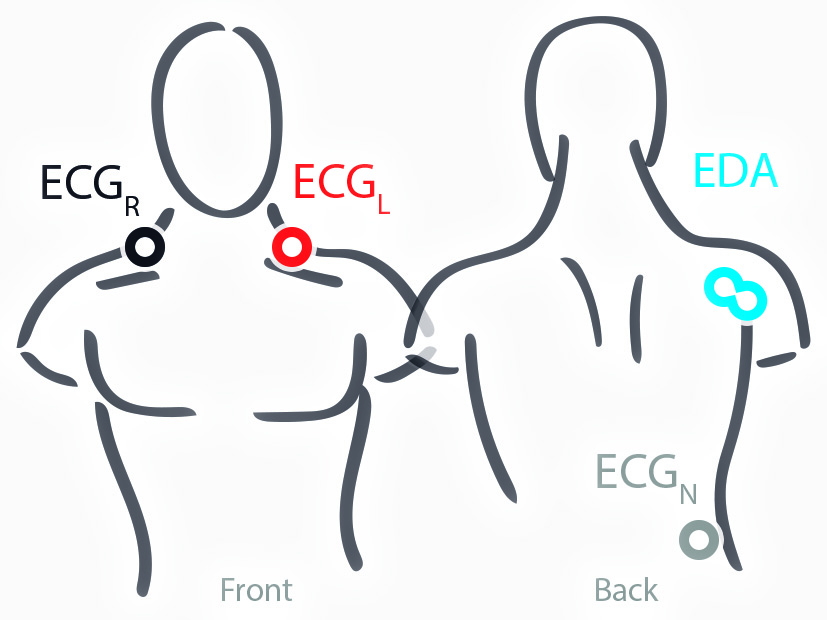
\includegraphics[width=\textwidth]{include/images/electrodes.jpg}
		\caption{Schematische Übersicht zur Platzierung Elektroden für ECG (Herzschlag) und EDA (Hautleitfähigkeit) in Anlehnung an \textcite{ECGLeadPlacement2015}}
		\label{fig:electrodes-schema}
	\end{subfigure}
	\label{fig:biosignals}
\end{figure}
\end{frame}

\subsection{Ergebnisse}

\begin{frame}{\currentname{} -- Teilnehmer*innen}
	\begin{itemize}[label=\textcolor{tertiary}{\faicon{caret-right}}]
		\item 28 (13 w, 15 m) Teilnehmer*innen, 
		\item Alter: 30,7 Jahre (SD = 10.6)
		\item Können: Vorstieg (23), 6+ (± 1 Grad); Top-Rope (5), 5+/6- (±1 Grad) \textcolor{source}{Skala: UIAA}
		\item VR Vorerfahrung: keine (13), minimal (13), selten (2)
		\item keine überdurchschnittliche Ängstlichkeit (nach STAI-T)
		\item keine klinische Höhenangst (nach vHI)
	\end{itemize}
\end{frame}

\begin{frame}{\currentname{} -- Vergleichbarkeit}
\begin{tabbing}
	\textcolor{primary}{\faicon{question-circle}} \quad \= Welchen Effekt hat die Bedingung (Griffe/Tritte|Controller) auf Präsenz/Angst?
\end{tabbing}
	\only<2->{\begin{figure}[htb]
	\centering
	\begin{subfigure}[t]{0.49\columnwidth}
		\centering
		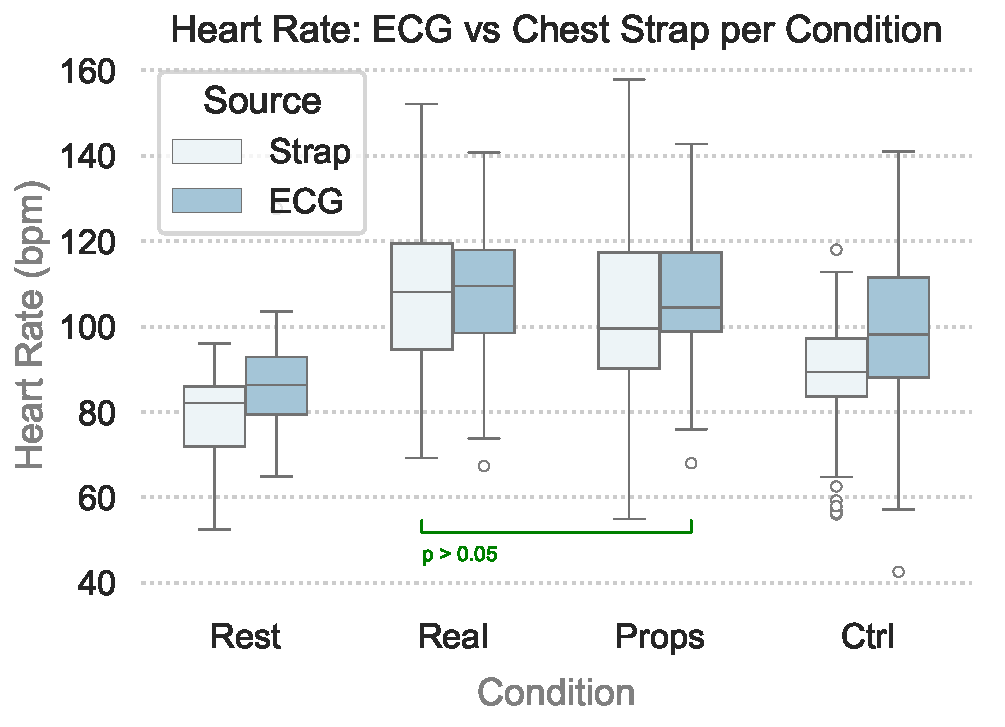
\includegraphics[width=\textwidth]{include/images/hr_per_condition_by_source.pdf}
		\label{fig:physical-exertion-hr}
	\end{subfigure}
	\hspace*{\fill}
	\begin{subfigure}[t]{0.49\columnwidth}
		\centering
		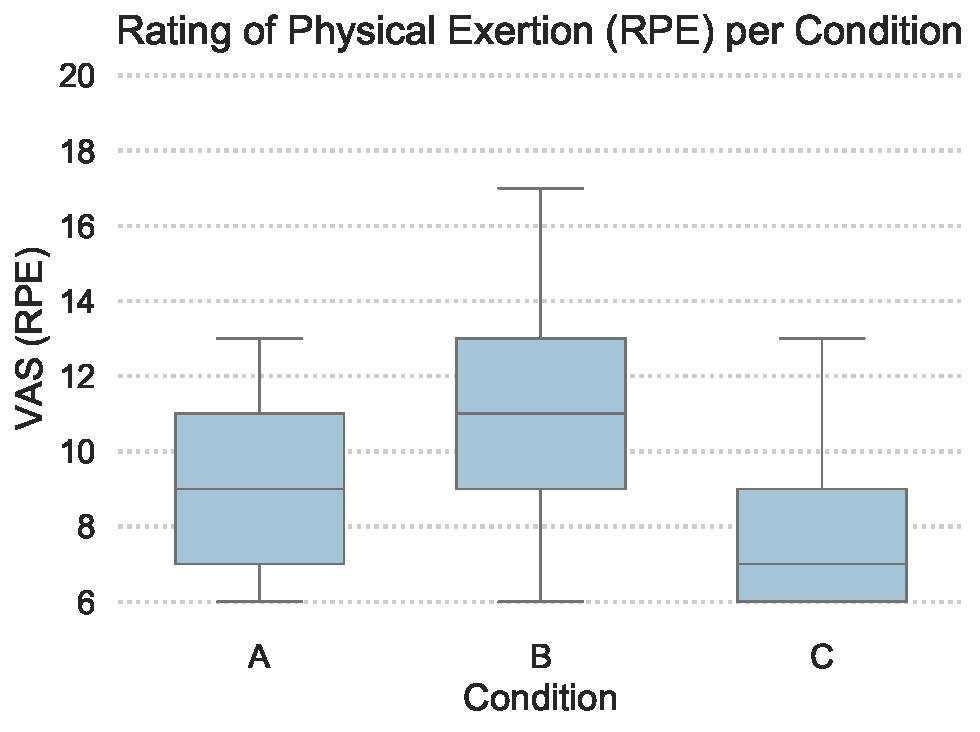
\includegraphics[width=\textwidth]{include/images/rpe_per_condition.pdf}
		\label{fig:physical-exertion-rpe}
	\end{subfigure}
	\label{fig:physical-exertion}
\end{figure}}
\end{frame}

\begin{frame}{\currentname{} -- Angst}
\begin{figure}[htb]
	\centering
	\begin{subfigure}[t]{0.49\columnwidth}
		\centering
		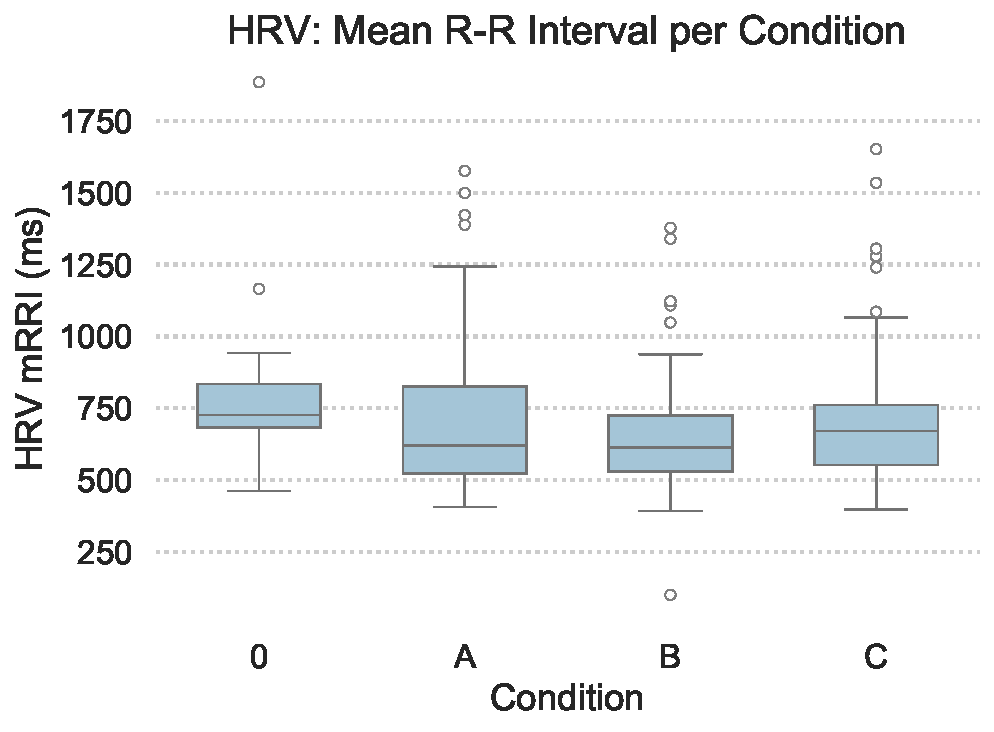
\includegraphics[width=\textwidth]{include/images/hrv_per_condition.pdf}
		\label{fig:stress-hrv}
	\end{subfigure}
	\hspace*{\fill}
	\begin{subfigure}[t]{0.49\columnwidth}
		\centering
		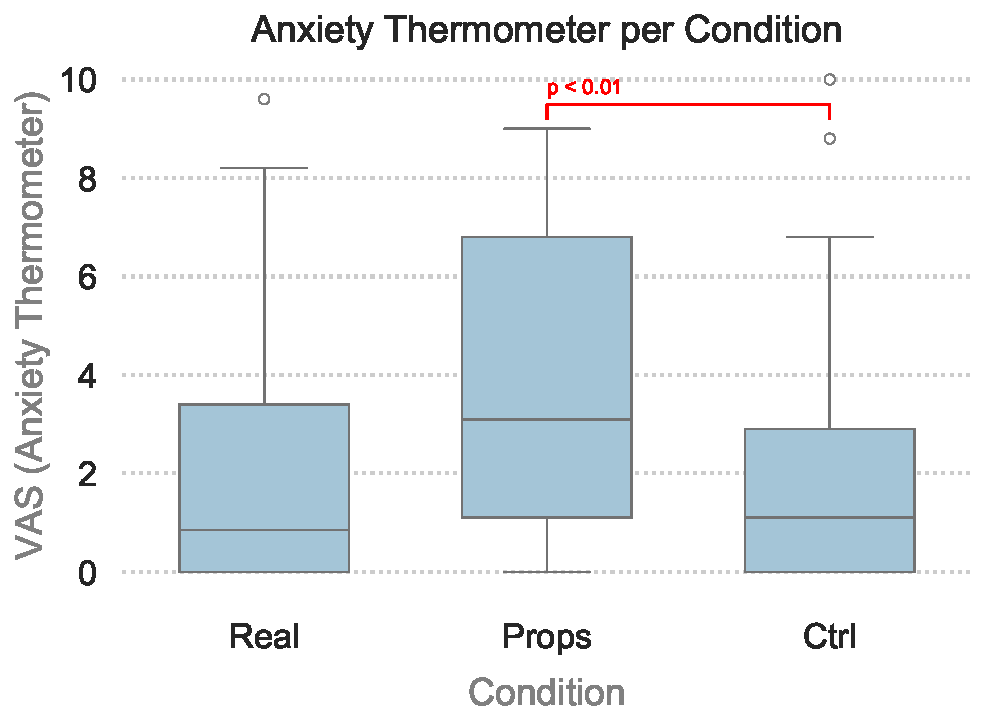
\includegraphics[width=\textwidth]{include/images/at_per_condition.pdf}
		\label{fig:anxiety-at}
	\end{subfigure}
	\label{fig:stress-anxiety}
\end{figure}
\end{frame}

\begin{frame}{\currentname{} -- Präsenz}
\begin{figure}[htb]
   \begin{center}
   	   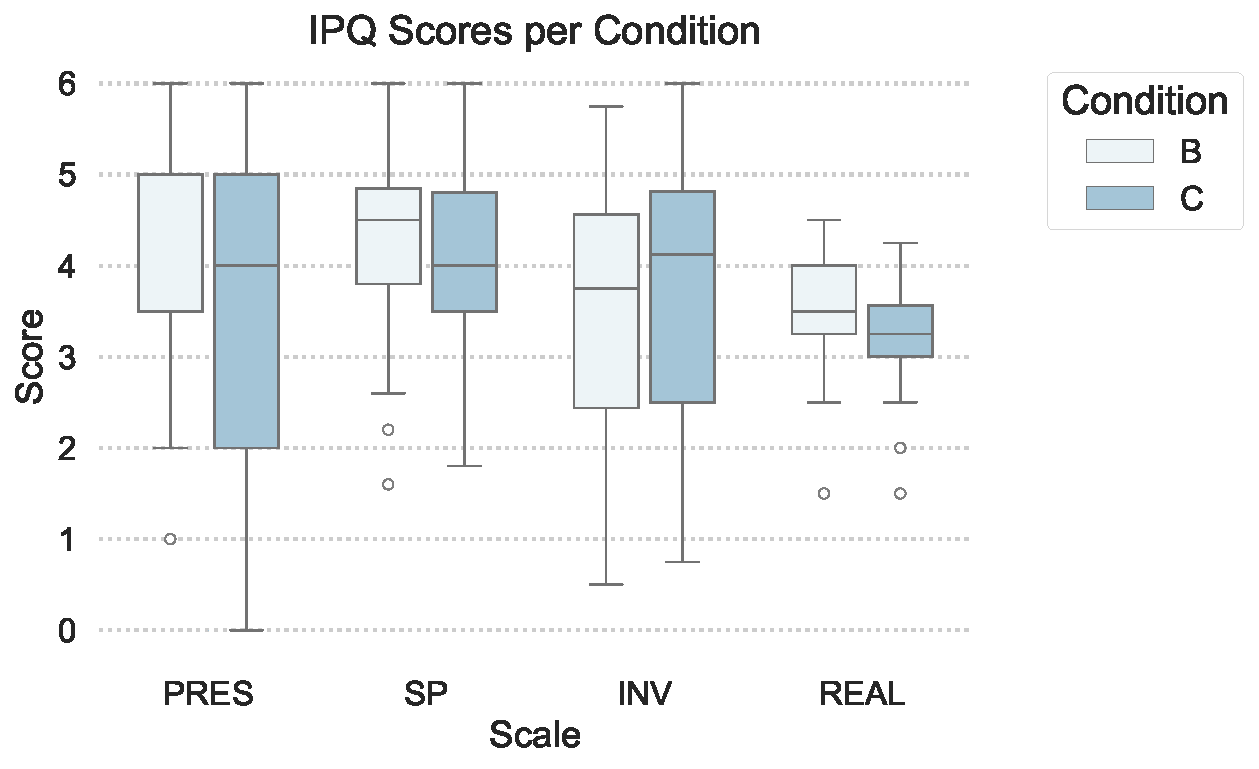
\includegraphics[width=0.6\textwidth]{include/images/ipq_per_condition}
   	\captionsetup{subrefformat=parens}
   	\caption{\gls{IPQ} Werte für die Bedingungen B und C auf den Skalen \textit{general presence} (PRES), \textit{spatial awareness} (SP), \textit{involvement} (INV), and \textcolor{secondary}{\textit{realness} (REAL)}}
   	\label{fig:presence}
   \end{center}
\end{figure}
\end{frame}

\subsection{Diskussion}

\begin{frame}{\currentname{} -- Mehrdeutigkeit}
\begin{tabbing}
	\textcolor{primary}{\faicon{question-circle}} \quad \= Welchen Effekt hat die Bedingung (Griffe/Tritte|Controller) auf Präsenz/Angst?
\end{tabbing}
\begin{description}
	\item[Präsenz/Angst]\mbox{}
	\begin{itemize}
		\item[\textit{Psych.}] Griffe/Tritte $\rightarrow$ \textbf{erhöhte} Präsenz u. Angst
		\item[\textit{Phys.}] \textbf{kein Unterschied} messbar zw. Griffe/Tritte|Controller
	\end{itemize}
\end{description}
\end{frame}

\begin{frame}{\currentname{} -- Welche Angst?}
\begin{description}
	\item[Selbstwahrnehmung]\mbox{}
	\begin{itemize}[label=\textcolor{tertiary}{\faicon{caret-right}}]
		\item Auslöser unklar, nicht zwingend Sturzangst
		\item Alternativer Ursprung: Unsicherheit mit VR System
	\end{itemize}
	\item[Biosignale]\mbox{}
	\begin{itemize}[label=\textcolor{tertiary}{\faicon{caret-right}}]
		\item Hautleitfähigkeit zeigt keine konsistente Veränderung
		\item Vermutung: Durchschnittswerte unpassend; Bewegungsartefakte
	\end{itemize}
\end{description}
\end{frame}

\section{Fazit und Ausblick}

\begin{frame}{\currentname{}}
	\textbf{Höhen-, Flug-, \textcolor{secondary}{und Sturzangst?}}
	\begin{itemize}[label=\textcolor{tertiary}{\faicon{caret-right}}]
		\item Ja und nein $\rightarrow$ mehr Forschung nötig zu Angst + physische Aktivität
	\end{itemize}
	\textbf{Technologischer Mehrwert}
	\begin{itemize}[label=\textcolor{tertiary}{\faicon{caret-right}}]
		\item neuartige, präzise Darstellung von Händen in VR zur physischen Interaktion
	\end{itemize}
	\vfill{}
	\hfill{}\textit{VR \xcancel{Therapie} Training für Sturzangst bleibt Zukunftsmusik} \textcolor{secondary}{\faicon{sign-out}}
\end{frame}

\begin{frame}[plain]
\begin{center}
	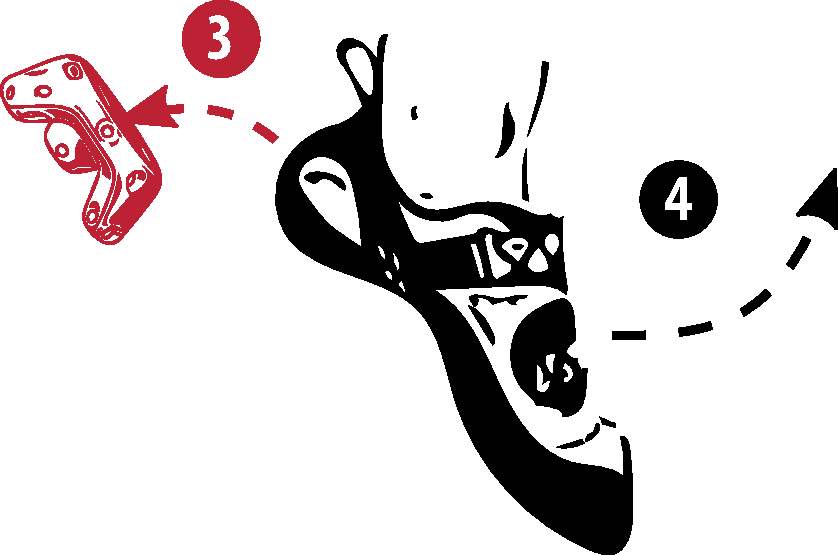
\includegraphics[width=0.8\textwidth]{include/images/climbing-shoe-with-instructions-off.pdf}
\end{center}
\end{frame}


\appendix

\begin{frame}[allowframebreaks]{Literaturverzeichnis}

\printbibliography[heading=none]

\end{frame}

\backupbegin

\begin{frame}{Eigene Forschungsprojekte -- Imagery in Sport Climbing}
\begin{figure}[h]
	\centering
	\begin{subfigure}[t]{0.49\columnwidth}
		\centering
		\begin{overpic}[width=\textwidth]{include/images/Google-Glass.jpg}
			\rbox{-1}{1}{\textcolor{source}{\tiny{Quelle: \href{https://de.wikipedia.org/wiki/Datei:Google_Glass_Main.jpg}{Wikipedia}}}}
		\end{overpic}
		\label{fig:google-glass}
	\end{subfigure}
	\hspace*{\fill}
	\begin{subfigure}[t]{0.49\columnwidth}
		\centering
		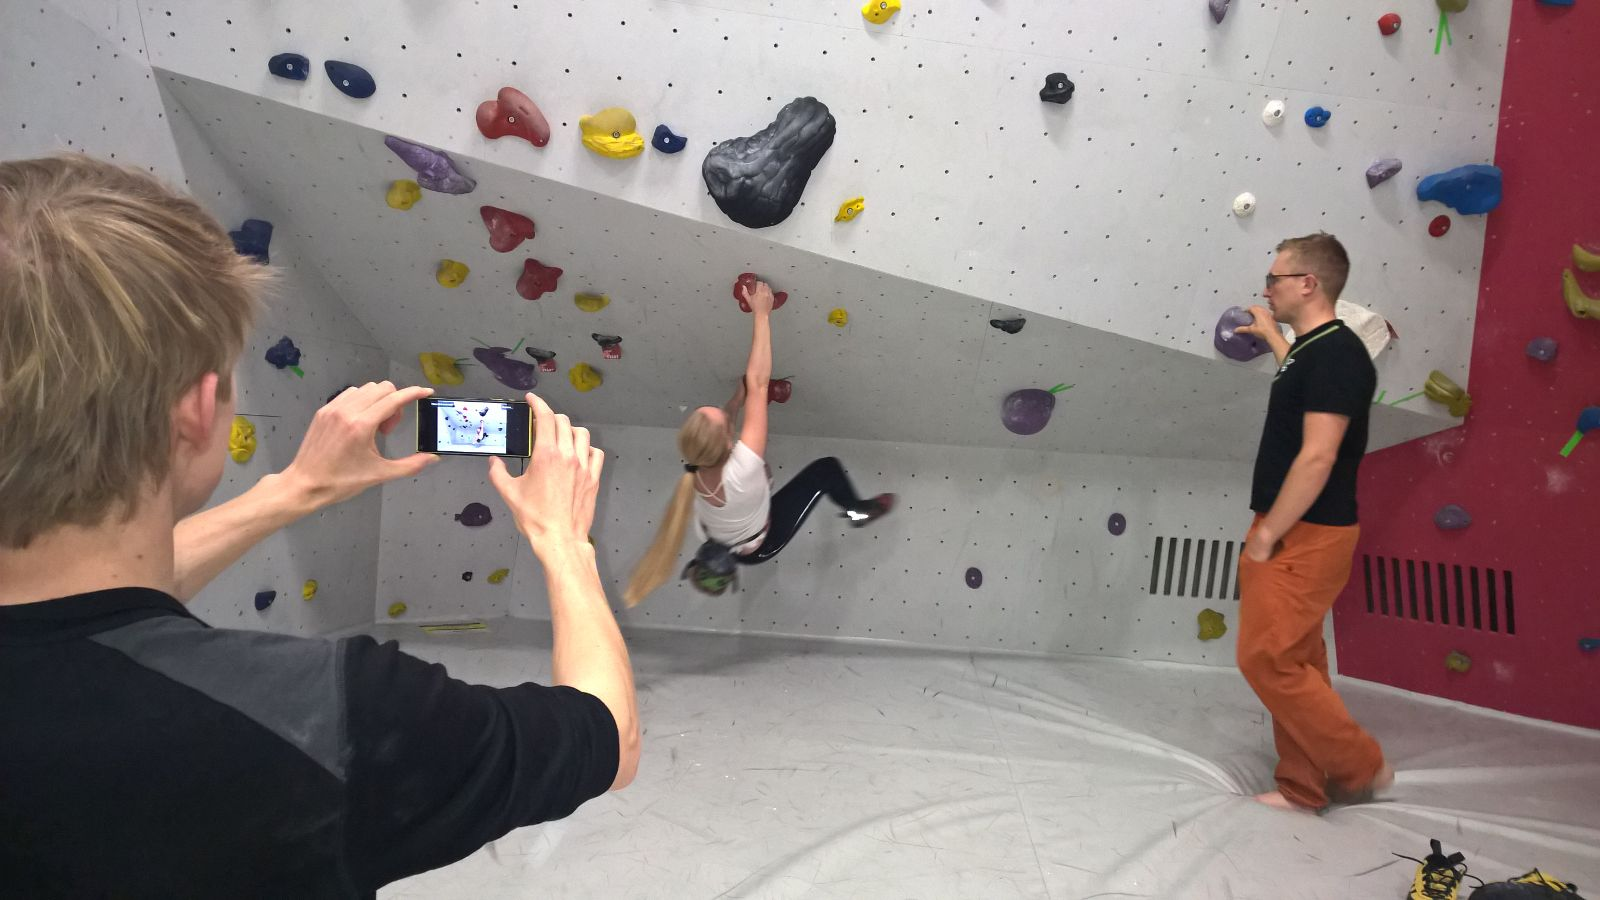
\includegraphics[width=\textwidth]{include/images/Live-Video.jpg}
		\label{fig:live-video-action}
	\end{subfigure}
	\caption{Livebildübertragung vom Smartphone (Kamera) an Google Glass Brille (Display). \\Die Kletterin kann sich selbst beim Klettern sehen, während sie klettert.}
	\label{fig:live-video}
\end{figure}
\end{frame}

\begin{frame}{Eigene Forschungsprojekte -- Crimp\textcolor{tertiary}{Bit}}
\begin{figure}[h]
\centering
\begin{subfigure}[t]{0.35\columnwidth}
	\centering
	\begin{overpic}[width=\textwidth]{include/images/myo-armband.jpg}
		\rbox{-9}{1}{\textcolor{source}{\tiny{Quelle: \href{https://www.myo.com}{Thalmic Labs Inc.}}}}
	\end{overpic}
	\label{fig:myo-armband}
\end{subfigure}
\hspace*{\fill}
\begin{subfigure}[t]{0.62\columnwidth}
	\centering
	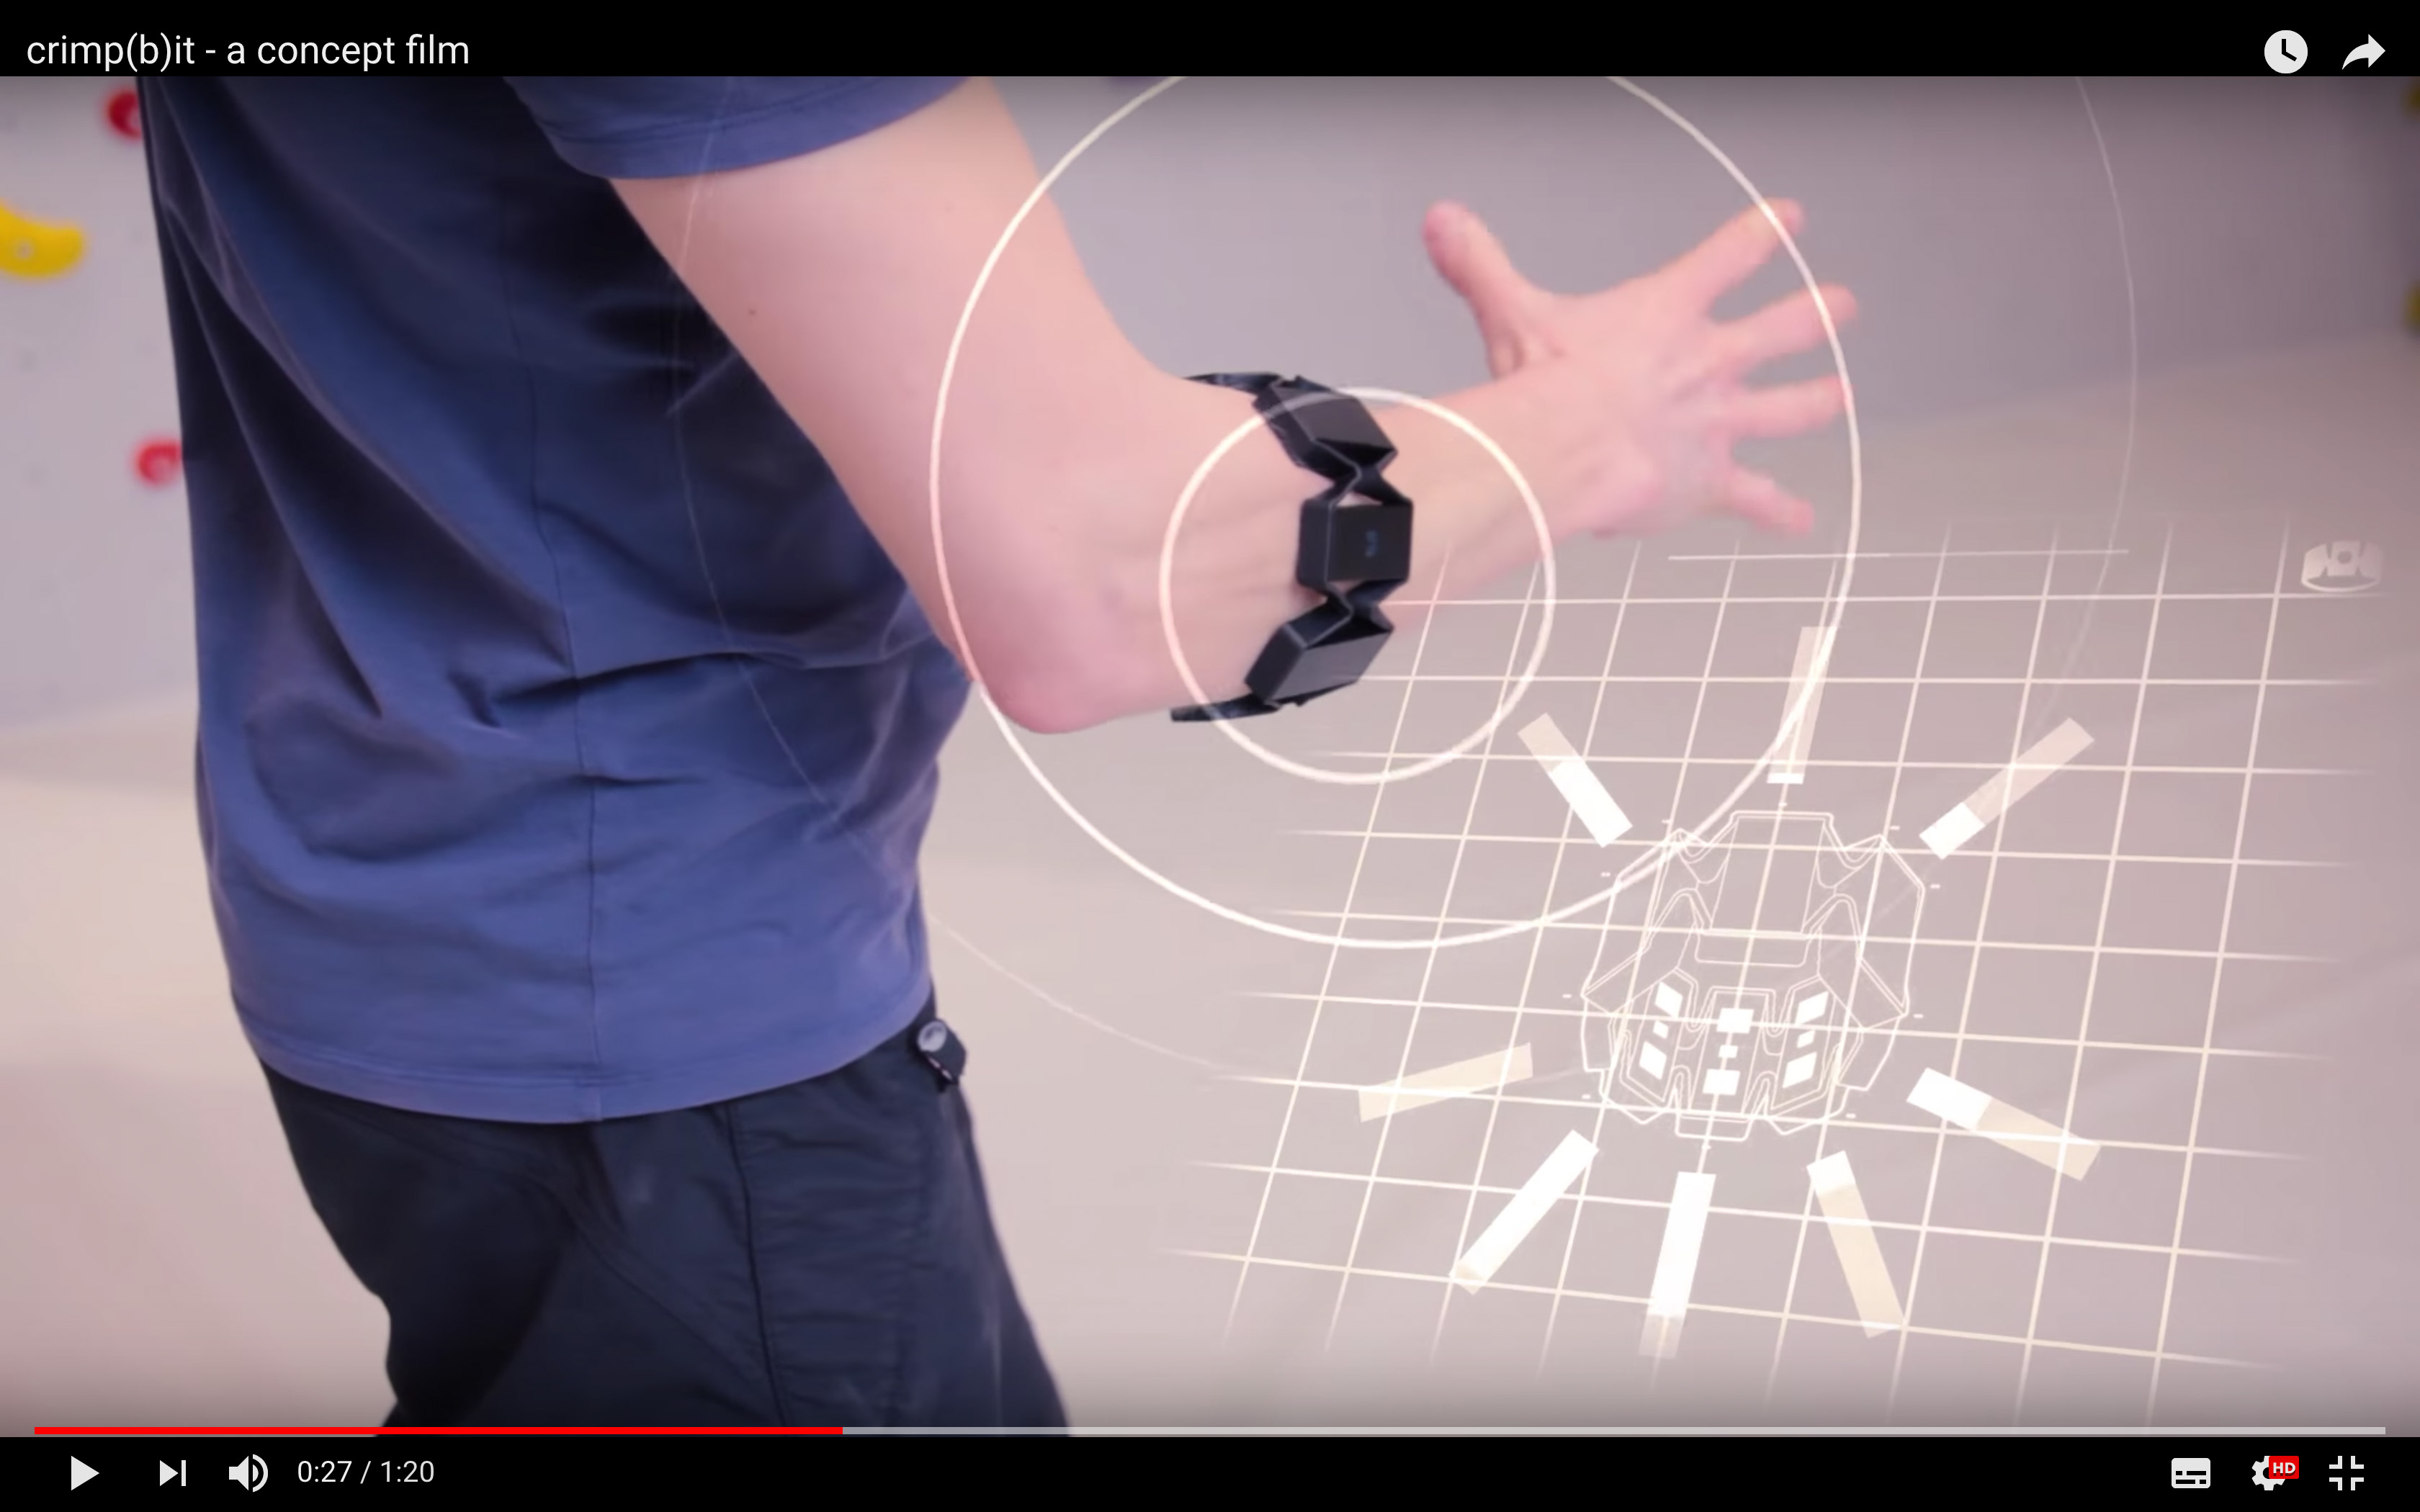
\includegraphics[width=\textwidth]{include/images/myo-demo.jpg}
	\label{fig:crimpbit-demo}
\end{subfigure}
\caption{MYO Armband zur Gestenerkennung als Sensor für potentiell schädliche Greifbewegungen.}
\label{fig:crimpbit}
\end{figure}
\end{frame}

\begin{frame}{Related Work mit \textit{Höhen} und \textit{Kanten}}
\begin{columns}
	\begin{column}{0.45\textwidth}
		\begin{center}
			\begin{overpic}[height=0.8\textheight]{include/images/pijpers.jpg}
				\rbox{-15}{1}{\textcolor{black}{\tiny{Quelle: \href{https://www.researchgate.net/figure/Side-view-of-the-virtual-environment-Subjects-start-in-the-Training-Room-and-later-enter_fig1_247181822}{ResearchGate}}}}
			\end{overpic}
		\end{center}
	\end{column}
	\begin{column}{0.55\textwidth}
		\begin{center}
			\begin{overpic}[height=0.8\textheight]{include/images/meehan.jpg}
				\rbox{-1}{1}{\textcolor{source}{\tiny{Quelle: \href{https://www.researchgate.net/figure/View-of-the-20-in-pit-from-the-wooden-ledge_fig3_7596875}{ResearchGate}}}}
			\end{overpic}
		\end{center}
	\end{column}
\end{columns}
\end{frame}

\begin{frame}{\currentname{} -- Teilnehmer*innen}
\begin{itemize}[label=\textcolor{tertiary}{\faicon{caret-right}}]
	\item 28 (13 w, 15 m) Teilnehmer*innen, 
	\item Alter: 30,7 Jahre (SD = 10.6)
	\item Können: Vorstieg (23), 6+ (± 1 Grad); Top-Rope (5), 5+/6- (±1 Grad) \textcolor{source}{Skala: UIAA}
	\item VR Vorerfahrung: keine (13), minimal (13), selten (2)
	\item keine überdurchschnittliche Ängstlichkeit (nach STAI-T)
	\item keine klinische Höhenangst (nach vHI)
\end{itemize}
\end{frame}

\begin{frame}{\currentname{} -- Vergleichbarkeit}
\begin{tabbing}
\textcolor{primary}{\faicon{question-circle}} \quad \= \large Welchen Effekt hat die Bedingung (Griffe/Tritte|Controller) auf Präsenz/Angst?
\end{tabbing}
\begin{figure}[htb]
	\centering
	\begin{subfigure}[t]{0.49\columnwidth}
		\centering
		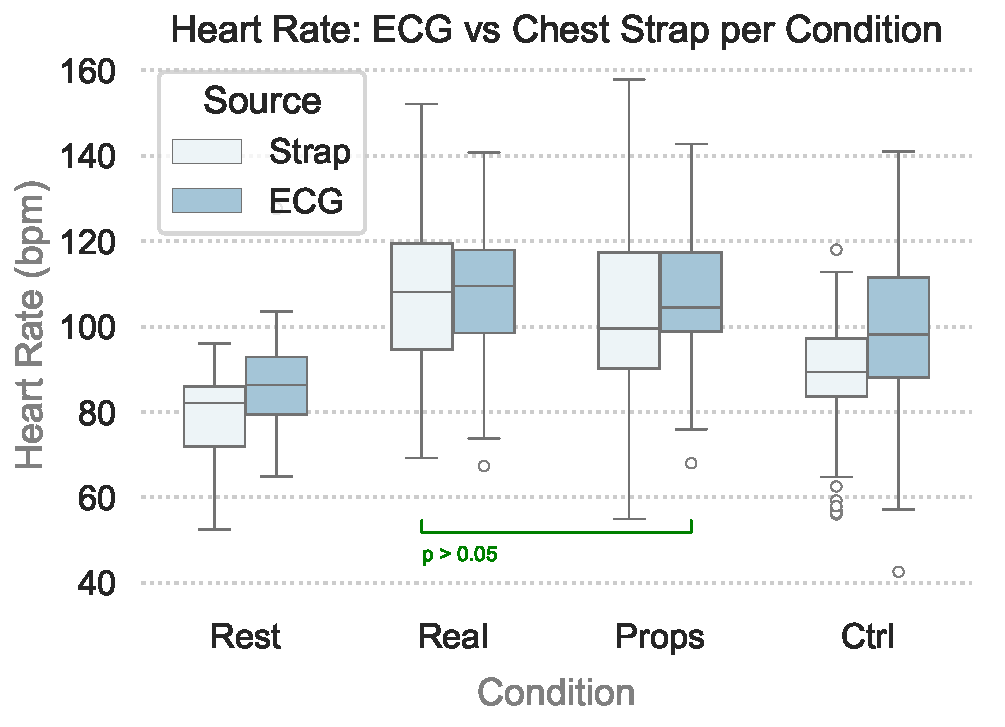
\includegraphics[width=\textwidth]{include/images/hr_per_condition_by_source.pdf}
		\label{fig:physical-exertion-hr}
	\end{subfigure}
	\hspace*{\fill}
	\begin{subfigure}[t]{0.49\columnwidth}
		\centering
		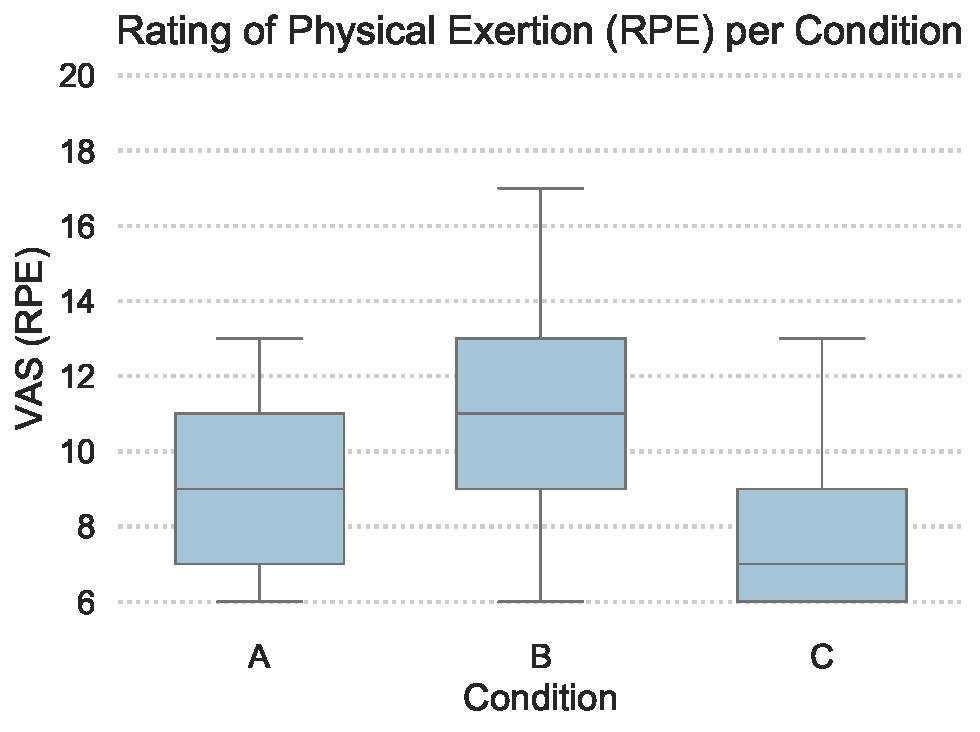
\includegraphics[width=\textwidth]{include/images/rpe_per_condition.pdf}
		\label{fig:physical-exertion-rpe}
	\end{subfigure}
	\label{fig:physical-exertion}
\end{figure}
\end{frame}

\begin{frame}{Vokabular: Immersion, Präsenz und Angst}
\begin{description}
	\item[Immersion]<2-> Die technischen Möglichkeiten in ein virtuelle Welt einzutauchen,\\z.B. Bildschirm, grafische Darstellung, Ton \autocite{McMahan2003}
	\item[Präsenz]<2-> Das aus Immersion resultierende Gefühl, vor Ort zu sein \autocite{McMahan2003}
	\item[Angst] Mehrdimensionales Phänomen: Psych. u. Phys. Symptome \autocite{Krohne1996}
	\item[Sturzangst] Angst vor dem Unkontrollierten, einer Verletzung \autocite{Lewis2010}
\end{description}
\begin{center}
	\only<3->{\large\textbf{Angeonommener Zusammenhang}\\Immersion $\sim$ Präsenz $\sim$ Angst }
\end{center}
\end{frame}

\begin{frame}{Forschungsfrage}
\begin{center}
\LARGE
$\substack{\text{Immersion}\\(\text{variieren})} \sim \substack{\text{Präsenz}\\(\text{messen})} \sim \substack{\text{Angst}\\(\text{messen})}$
\end{center}
\metroset{block=fill}
\begin{center}
\begin{minipage}{0.7\textwidth}
	\begin{block}{Alternativ-Hypothese (H\textsubscript{a}\label{hyp:anxiety})}<2->
		Das \textcolor{tertiary}{Präsenz}erleben von KletterInnen in \gls{VR} \textbf{steigt} wenn sie sich tatsächlich festhalten müssen, da dies die \textcolor{tertiary}{Immersion} \textbf{erhöht} und damit die \textcolor{tertiary}{Angst} \textbf{vergrößert}.
	\end{block}
	\begin{block}{Null-Hypothese (H\textsubscript{0}\label{hyp:anxiety})}<2->
		Es gibt keinen messbaren Unterschied zwischen Klettern in \gls{VR} mit \textcolor{tertiary}{Griffen und Tritten} gegenüber Klettern in \gls{VR} mit \textcolor{tertiary}{Game Controllern}.
	\end{block}
\end{minipage}
\end{center}
\end{frame}

\subsection{Diskussion}

\begin{frame}{\currentname{} -- Mehrdeutigkeit}
\begin{tabbing}
	\textcolor{primary}{\faicon{question-circle}} \quad \= \Large Wie wirken Griffe/Tritte|Controller auf \textcolor{secondary}{Realitätsempfinden} und \textcolor{secondary}{Angst}?
\end{tabbing}
{
	\setlength{\leftmargini}{2.15cm}
	
	\begin{itemize}
		\item[\textcolor{secondary}{\textit{subjektiv}}] Griffe/Tritte $\rightarrow$ \textbf{erhöhte}(s) Realitätsempfinden und Angst\\
		\temporal<2>{\textcolor{white}{...}}{\textcolor{secondary}{Auslöser unklar, nicht zwingend Sturzangst}}{\textcolor{gray}{Auslöser unklar, nicht zwingend Sturzangst}}
		\item[\textcolor{secondary}{\textit{messbar}}] \textbf{kein Unterschied} messbar zw. Griffe/Tritte|Controller\\
		\temporal<3>{\textcolor{white}{...}}{\textcolor{secondary}{Ursache unklar, Messgrößen/-Verfahren möglicherweise ungeeignet}}{Ursache unklar, Messgrößen/-Verfahren möglicherweise ungeeignet}
	\end{itemize}
}
\end{frame}

\backupend
	
\end{document}